\documentclass[b5paper, 11pt, norsk]{MScthesisITEM}

% this package is just to generate text for demo-purposes
\usepackage[norsk]{babel}
%\usepackage{blindtext}
\usepackage{parskip}

\usepackage{tikz}
\usepackage{adjustbox}
\usetikzlibrary{shapes,snakes}
\usepackage{amsmath,amssymb}
\usepackage{sidecap}
\usepackage{multirow}


\title{Distribusjon av informasjon for økt  \newlinetitle awareness i et avbruddsdrevet miljø} % The title of your assignement; NB use \newlinetitle to start a newline
\author{Veronica Sund \\ \newlinetitle Monika Hafredal} % Your firstname and lastname
\professor{Lill Kristiansen, ITEM} % Affiliation = ITEM for instance
\supervisor{Joakim Klemets, ITEM}
\date{Desember 2013}

%% Uncomment the following in case you want subfigures; note that there will be a warning for the caption package
 \let\subcaption\undefined
 \let\subfloat\undefined
 \usepackage[bf]{caption}
 \usepackage{subcaption}

\DeclareGraphicsExtensions{.pdf,.jpg,.png}
\graphicspath{{./figs/}}


\loadglsentries{glossary}
\makeglossaries

\begin{document}
\selectlanguage{norsk}
\pagenumbering{roman}
\pagestyle{plain}

%% Only for the project
\titleITEM

%% Only for the master's thesis; for the project report the description is taken from It's Learning and added by the department
% \selectlanguage{english} % Change to 'norsk' if you are writing in Norwegian
% \input{problem_description}
% \cleardoublepage

%% There must be an abstract in English, even though the main text is in Norwegian
\selectlanguage{english}
\pagestyle{empty}
\begin{abstract}

\noindent
To maintain awareness of colleagues' work is essential for good coordination. Nurses receive information necessary to maintain such awareness through external interrupts. These disruptions, in addition to the already interrupted-driven environment they work in.
This research paper looks at the nurse call system at St. Olav's Hospital in Trondheim. We have seen how this works today, how nurses maintain awareness at work item and how it interrupted-driven environment affects their work.


%\Blindtext[5][1]
\end{abstract}
\cleardoublepage

%% Only for the master's thesis; if the main text is in English and you can write Norwegian, there must be an abstract in Norwegian as well.A
\selectlanguage{norsk}
\pagestyle{empty}
\renewcommand{\abstractname}{Sammendrag}
\begin{abstract}
\noindent Sikkerheten til nesten all offentlig nøkkel-kryptografi er basert på et vanskelig beregnbarhetsproblem. Mest velkjent er problemene med å faktorisere heltall i sine primtallsfaktorer, og å beregne diskrete logaritmer i endelige sykliske grupper. I de to siste tiårene, har det imidlertid dukket opp en rekke andre offentlig nøkkel-systemer, som baserer sin sikkerhet på helt andre type problemer. Et lovende forslag, er å basere sikkerheten på vanskeligheten av å løse store likningsett av flervariable polynomlikninger. En stor utfordring ved å designe slike offentlig nøkkel-systemer, er å integrere en effektiv ``falluke'' (trapdoor) inn i likningssettet. En ny tilnærming til dette problemet ble nylig foreslått av Gligoroski m.f., hvor de benytter konseptet om kvasigruppe-strengtransformasjoner (quasigroup string transformations). I denne masteroppgaven beskriver vi en metodikk for å identifisere sterke og svake nøkler i det nylig foreslåtte multivariable offentlig nøkkel-signatursystemet MQQ-SIG, som er basert på denne idéen.

Vi har gjennomført et stort antall eksperimenter, basert på Gröbner basis angrep, for å klassifisere de ulike parametrene som bestemmer nøklene i MQQ-SIG. Våre funn viser at det er store forskjeller i viktigheten av disse parametrene. Metodikken består i en klassifisering av de forskjellige parametrene i systemet, i tillegg til en innføring av konkrete kriterier for hvilke nøkler som bør velges. Videre, har vi identifisert et unødvendig krav i den originale spesifikasjonen, som krevde at kvasigruppene måtte oppfylle et bestemt kriterie. Ved å fjerne denne betingelsen, kan nøkkel-genererings-algoritmen potensielt øke ytelsen med en stor faktor. Basert på alt dette, foreslår vi en ny og forbedret nøkkel-genereringsalgoritme for MQQ-SIG, som vil generere sterkere nøkler og være mer effektiv enn den originale nøkkel-genereringsalgoritmen.  
\end{abstract}
\cleardoublepage

%\selectlanguage{english}% Change to 'norsk' if you are writing in Norwegian
%\pagestyle{empty}
\begin{abstract}

\noindent
To maintain awareness of colleagues' work is essential for good coordination. Nurses receive information necessary to maintain such awareness through external interrupts. These disruptions, in addition to the already interrupted-driven environment they work in.
This research paper looks at the nurse call system at St. Olav's Hospital in Trondheim. We have seen how this works today, how nurses maintain awareness at work item and how it interrupted-driven environment affects their work.


%\Blindtext[5][1]
\end{abstract}


\renewcommand{\abstractname}{Preface}
\begin{abstract}

\noindent
Denne prosjektoppgaven er skrevet ved Institutt for Telematikk (ITEM) ved Norges Teknisk-Naturvitenskapelige Universitet (NTNU), høsten 2013. Forfatterene har fulgt studieprogrammet Kommunikasjonteknologi innen retingen Nett og Tjenester, med fordypning innen Telematikk og Samfunn. 

\noindent
Bakgrunnsinformasjon og -data er skaffet gjennom studier av tidligere arbeid, samt workshops med test og evaluering av prototype. 

\noindent
Vi vil først takke professor Lill Kristiansen (ITEM), ansvarlig professor for oppgaven, for gode innspill underveis. Vi ønsker også å rette en stor takk til vår veileder Ph.D. kandidat Joakim Klemets, ved ITEM, for gode tilbakemeldinger, konstruktiv kritikk og støtte underveis i arbeidet. Joakim la også stor innsats i å skaffe deltagere til workshopene.

\noindent
Vi vil også takke Terje Røsand ved Norsk Senter for Elektronisk Pasientjournal (NSEP) for gode videoopptak av workshopene, og god veiledning i forkant av disse. Til sist vil vi takke alle som har brukt tid på å hjelpe oss å lese korrektur på oppgaven.

\centering

Trondheim, 11. desember 2013\\
Veronica Sund\\
Monika Hafredal

%\blindtext 
\end{abstract}
\cleardoublepage

% similarly you may add a separate acknowledgments page

\tableofcontents*
\cleardoublepage


%% include if relevant
\listoffigures
\cleardoublepage

%% include if relevant
\listoftables
\cleardoublepage

%% include if relevant
%\listofalgorithms
%\addcontentsline{toc}{chapter}{List of Algorithms}
\cleardoublepage

%% include if relevant
%\printglossary[title=List of Symbols, style=long]
\cleardoublepage
%\glsaddall[]

%% include if relevant
%\printglossary[title=List of Acronyms,type=\acronymtype] % prints just the list of acronyms
\cleardoublepage

\pagenumbering{arabic}
\pagestyle{ruled}
\include{Introduksjon}
\chapter{Teori}
\label{chp:teori}


Vi vil i dette kapittelet presentere teori relevant for vår forskning. Denne teorien er et resultat av kvalitative literaturstudier, en metode nærmere beskrevet i kapittel \ref{chp:forskningsmetode}. Vi har valgt å fokusere på temaer vi mener er sentrale for spørsmålene vi søker svar på. Da vår oppgave omhandler et system som skal støtte samarbeid i et høyst dynamisk miljø, inneholder denne delen  både menneskelige og organisatoriske aspekter, samt teori knyttet til design og utvikling av slike systemer.

\section{Kognitiv distribusjon og kapasitet}
\label{chp: kognisjon}

Ofte vil arbeidsaktiviteter bestå av flere sammenflettede oppgaver i en gitt tidsramme. Jo lenger tid det tar å utføre en oppgave, jo større sjanse er det for at andre oppgaver eller handlinger må utføres i løpet av denne perioden. Disse oppgavene kan ha ulik avbruddsverdi - prioritet, personlig- eller sosial viktighet, hastegrad ol. \cite{Rogers94}. 
Da CSCW kom mot slutten av 80-tallet, oppsto utfordringene om hvordan datasystemer bør designes for å støtte grupper av individer som kommuniserer og arbeider sammen \cite{Rogers94}. 

\tikzstyle{mybox} = [draw=black, fill=white, very thick,
    rectangle, inner sep=10pt, inner ysep=20pt, rounded corners]
\tikzstyle{fancytitle} =[fill=black, text=white]
\begin{tikzpicture}
\node [mybox] (box){%
    \begin{minipage}{0.9\textwidth}
     Computer-Supported Cooperative Work er et tverrfaglig område hvor forskere studerer hvordan grupper av samarbeidende mennesker jobber, og hvordan teknologi kan være til støtte for arbeidet. CSCW-teknologi defineres som PC-baserte systemer som støtter grupper av mennesker engasjert i en felles oppgave, eller med et felles mål, og som gir et grensesnitt til det delte miljøet (Ellis (1991)) \nocite{Ellis91}.
    \end{minipage}
};
\node[fancytitle, rounded corners, right=10pt] at (box.north west) {CSCW};
\end{tikzpicture}%


\noindent
Gitt at mange arbeidsaktiviteter er kognitive, de krever tenkning, problemløsing og evne til å forutse og ta beslutninger, argumenterer Rogers og Ellis (1994) for at det kreves en forståelse for hvordan disse aktivitetene utføres for å kunne designe datasystemer som kan støtte både kognitive aktiviteter og sosial interaksjon.

\tikzstyle{mybox} = [draw=black, fill=white, very thick,
    rectangle, inner sep=10pt, inner ysep=20pt, rounded corners]
\tikzstyle{fancytitle} =[fill=black, text=white]
\begin{tikzpicture}
\node [mybox] (box){%
    \begin{minipage}{0.9\textwidth}
     Det som har med erkjennelse, oppfatning og tenkning å gjøre. I filosofi og psykologi opptrer ofte uttrykket 'kognitiv' som motsetning til det følelsesmessige eller intuitive. Et kognitivt system er et som kan behandle en viss type informasjon, for eksempel sanseinntrykk, minner, tanker eller språk. Menneskehjernen regnes som et eksempel på et kognitivt system (Malt et al. (2013), Store medisinske leksikon).
    \end{minipage}
};
\node[fancytitle, rounded corners, right=10pt] at (box.north west) {Kognitiv};
\end{tikzpicture}%

\subsection{Kognitiv kapasitet}
“Stacking” defineres av Ebright (2010) som den usynlige beslutningsprosessen sykepleiere utfører om hva, hvordan og når de skal gi pleie til en tildelt gruppe pasienter. Stadige endringer i omgivelser og informasjonsflyt resulterer i en kontinuerlig re-prioritering av hvilke oppgaver man skal gjøre når. Dette kombinert med avbrytelser fra omgivelsene, kan resultere i en kognitiv belastning som kan hemme oppmerksomheten. Parker og Coiera (2000) hevder at en begrensende faktor i enhver kommunikasjonsanalyse er den kognitive kapasiteten individer har til å gjennomføre sitt arbeid, da studier har vist at feil og ineffektivitet er et resultat av at denne kapasiteten overskrides. Kunnskap om menneskets hukommelse hevdes å være nøkkelen til å forstå hvilke krav som bør settes til teknologi brukt i slike omgivelser. Det skilles normalt mellom langtids- og korttidsminne. Den passive kunnskapen man besitter ligger i langtidsminnet, for eksempel medisinske fakta eller viktige datoer, mens kortidsminnet, eller arbeidsminnet, er den bevisste delen av minnet som aktivt behandler informasjon. Arbeidsminnet har begrenset kapasitet og varighet, og lar seg raskt forstyrre av distraksjoner og avbrytelser. Coiera og Tombs (1998) \nocite{Coiera98} antyder at synkron kommunikasjon, ansikt-til-ansikt eller per telefon, foretrekkes fordi det gir en umiddelbar bekreftelse på at en beskjed er mottatt. Dersom man ønsker å gi en beskjed eller et ansvar videre, vil usikkerheten om beskjeden er mottatt bli liggende i arbeidsminnet frem til man får en bekreftelse fra mottaker. 




\section{Awareness}
\label{chp: awareness}

Et sykehus er en organisasjon hvor vi finner mange informasjonskilder, plutselig stress, rutinearbeid og ansatte som stadig er på forskjellige steder. Dette gjør at kommunikasjon er svært viktig for å sikre god pasientomsorg og -sikkerhet\cite{Klemets12}. Uttrykket funksjonsredundans (av det engelske 'redundancy of function') betyr at kunnskap om situasjonen til en hver tid er delt, og overlappende mellom medlemmene i gruppen.\cite{KlemetsRedundancy} Denne typen kunnskap kalles gjerne for bevissthet, og er et konsept med stadig større betydning, spesielt med tanke på CSCW \cite{Dourish92}. En slik bevissthet om andres aktiviteter er avgjørene for å sikre et vellykket samarbeid og god koordinasjon\cite{KlemetsRedundancy}. 

\subsubsection{Definisjoner og konseptualiseringer}
Bevissthet er et svært uklart og komplekst konsept med mange definisjoner og konseptualiseringer \cite{KlemetsRedundancy}\cite{Gutwin04}\cite{Schmidt02}. Begrepet bevissthet brukes i stadig flere sammenhenger, og mange forskere blir stedig mindre komfortable med å bruke begrepet i seg selv. For å komme til en slags konseptuell klarhet i hva bevissthet skal bety må vi innse at det ikke gir mening å se på bevissthet noe i seg selv, men må referere til en persons bevissthet \emph{om} noe \cite{Schmidt02}. Dermed har vi fått konsepter som blant annet sosial, eller kontekstformidlet sosial bevissthet \cite{Bardram04}, generell bevissthet\cite{Gross13}, romlig og tidsmessig bevissthet\cite{Randell}, gruppe-bevissthet\cite{Gutwin04}, perifer-, bakgrunns-, passiv- og gjensidig bevissthet\cite{Schmidt02}, noe som også gir mange forskjellige definisjoner. Dourish og Bellotti har definert begrepet som \emph{"...en forståelse av aktivitetene til andre, som gir kontekst for dine egne aktiviteter"}. En mer inngående definisjon finner vi i \cite{Endsly95}, som tar for seg konseptualliseringen situasjonell bevissthet: \emph{"Situasjonell bevissthet er oppfattelse av elemntene i omgivelsene avgrenset av tid og rom, forståelsen av deres mening, og prognosen for deres status i nær fremtid"}. i \cite{Gross13} er generell bevissthet definert som "den gjennomgripende opplevelsen av å vite hvem som befinner seg i nærheten, hva de driver med, om de er relativt opptatt eller kan engasjeres osv". Bardrams konsept kontekstformidlet sosial bevissthet har som mål å minimere uønskede forstyrrelser mellom mobile kolleger ved å øke deres sosiale bevissthet ved hjelp av kontekstbevisste systemer\cite{Bardram04}. Selv om begrepet bevissthet, som vi ser, ikke har en entydig definisjon er det viktig å legge merke til at bevissthet er en persons \emph{indre} kunnskap og forståelse av situasjonen\cite{Gross13}. 

\noindent
Bevissthet kan også deles inn i to kategorier, uavhengig av andre konseptualiseringer og definisjoner. (1) Biprodukt-bevissthet, hvor bevissthet oppnås uten at det krever merarbeid for brukerene, altså gjennom aktivitetene i seg selv, og motsettningen (2) bevissthet ved merarbeid, hvor kolleger må gjøre ekstra arbeid for å opprettholde bevissthet\cite{Randell}. 


\subsubsection{Bevissthet i CSCW}
Innen CSCW defineres bevissthet som det å "synliggjøre sine aktiviteter for, og oppfatte aktivitetene til kolleger, for å støtte opp om samarbeidet dem imellom". Bevissthet i denne sammenhengen ses på som essensiell for et godt samarbeid, og blir gjerne karakterisert som uanstrengt, eller biprodukt-bevissthet\cite{Randell}. 

\noindent
I følge både C. Heath et al. (2002) og Schmidt (2002), oppnås denne typen bevissthet gjennom kontinuerlig interaksjon med andre, og er på ingen måte en sinnstilstand eller passiv aktivitet. Dette underbygger tankene bak konseptualiseringen tilstandsbevissthet, hvor det kreves et visst nivå av kognitive ferdigheter for å til en hver tid kunne overvåke og oppdage endringer i omgivelsene. Dette skjer samtidig som man synliggjør for omgivelsene ens egen nåværende situasjon gjennom implisitte eller eksplisitte signaler. Med informasjonen man henter inn vil man da kunne danne seg et mentalt bilde av hvordan situasjonen til enhver tid er. I situasjoner hvor man ikke alltid er samlokalisert, som på et sykehus, kan bruk av kognitive gjenstander som whiteboards og skjermer være hensiktsmessig for å støtte opp under deling og innhenting av ovennevnte informasjon\cite{Bardram04}. 

\subsubsection{Bevissthet blant sykepleiere}
I \cite{Randell} foreslås tre konsepter av bevissthet som spesielt viktige i helseomsorgen. (1) Sosial bevissthet, som hvor kolleger befinner seg og deres aktiviteter, (2) romlig bevissthet, hva foregår på en gitt lokasjon, og (3) tidsmessig bevissthet, som omhandler tidligere, nåværende og fremtidige aktiviteter. 
Dette kan støttes ved bruk av kognitive gjenstander, og tar vi med oss definisjonen av bevissthet i forbindelse med CSCW som nevnt over ser vi at dette kan oppnås uten ekstra anstrengelser av sykepleierene.

\noindent
Selv om god pasientomsorg er avhengig av sykepleierenes oversikt over situasjonen til enhver tid må det også tas hensyn til pasienters og pårørendes privatliv. Får å opprettholde en god balanse mellom disse stilles det høye krav til sykepleierenes evne til å tilegne seg kunnskap om situasjonen på en måte som i minst mulig grad virker påtrengende for pasienter å pårørende, og at informasjon distribuert gjennom skjermer og tavler synlig for andre enn kun helsepersonell ikke krenker pasientenes privatliv\cite{Ebright10}.

\noindent
Da vi i denne oppgaven ser på bevisshet blant sykepleiere og deres bruk av kognitive gjenstander for å støtte opp om dette faller det seg naturlig å bruke definisjonen om bevissthet i CSCW. Derfor, når vi i denne oppgaven bruker begrepet bevissthet, vil det være denne definisjonen vi sikter til.

\section{Avbrudd}
\label{chp: avbrudd} 
\emph{Eksterne avbrytelser refererer til situasjoner hvor en ekstern hendelse fører til en forstyrrelse i prosessen med å fullføre en oppgave.} \cite{Harr07}

\subsubsection{Dualiteten ved avbrudd}
Grundgeiger og Sanderson (2009) skiller mellom \emph{gode} og \emph{dårlige} avbrudd, og hevder disse bør sees i sammenheng med hvilke effekter de har. Eksempler på positive effekter er awareness om perifer informasjon, øyeblikkelig kommunikasjon og tilgang til viktig informasjon. Avbryter opplever å få en umiddelbar bekreftelse på at informasjonen er mottatt og kan dermed avlaste arbeidsminnet, mens den som blir avbrutt kan oppleve en negativ effekt, eksempelvis at den kognitive kapasiteten overskrides, forsinkelse i eget arbeid, stress og frustrasjon. Samtidig kan avbruddet ha en positiv effekt dersom den som blir avbrutt mottar en alarm om en pasients alvorlige tilstand, eller annen ønsket informasjon.

\subsubsection{Avbruddshåndtering}
Gitt denne dualiteten, kan avbruddshåndtering sies å ha to mål: (1) redusere de negative effektene, og (2) utnytte de positive effektene av avbruddene. Harr og Kaptelinin (2007) og Grandhi og Jones (2010) gir fire teknikker for avbruddshåndtering:
\begin{enumerate}        
\item Forebygging - bruk av funksjoner som forebygger eller blokkerer innkommende avbrytelser, dette gjøres ofte enkelt ved å for eksempel skru av mobilen for en periode. En annen strategi er å kontrollere timingen til avbruddet, eller å kun tillate avbrytelser som er relevant for den oppgaven man utfører. Dette krever at awareness-informasjon er tilgjengelig, slik at timingen kan justeres for å minske den negative effekten ved avbruddet.

\item Fraråding - bruk av funksjoner som fraråder avbrytelser å oppstå, dette skjer ofte ved at man gir informasjon til avbryter om tilgjengeligheten til den denne ønsker å avrbyte. Harr og Kaptelinin (2007) presenterer konseptet om «availabilty management» (videre referert til som AM), definert som måten en person signaliserer til omgivelsene om han/hun er åpen for kommunikasjon eller ikke.
\noindent
Eksplisitt AM omhandler design av ulike typer teknisk støtte hvor brukere kan veksle mellom ulike tilgjengelighet/tilstedeværelse-profiler eller moduser. Implisitt AM benytter automatisk kalkulering, en strategi basert på automatisk innhenting  av informasjon fra ulike sensorer som eksempelvis måler lyd eller bevegelse. Denne informasjonen konverteres videre til signaler synlige for andre, for eksempel ved at ikoner skifter form eller farge.  

\item Modifiserte varslinger - bruk av funksjoner som modifiserer hvordan individer varsles om innkommende anrop. Ved bruk av ulike modaliteter som lyd, vibrasjon og lys, kan man minimere interferensen mellom perseptuelle og kognitive prosesser involvert i avbruddshåndtering og oppgaveytelse.

\item Forhåndsvisning - bruk av funksjoner som gir informasjon om selve avbrytelsen, som den avbrutte selv kan reflektere over.   
\end{enumerate}

\noindent
Forskere som arbeider innen \emph{interruption impact reduction}-paradigmet for avbruddshåndtering fokuserer på hvordan avbrytelser påvirker oppgaveytelse. Timing, frekvens, lengde og relevans til nåværende aktivitet eller oppgave er faktorer som påvirker de potensielle negative effektene avbruddet kan forårsake \citep{Grandhi10, Harr07}.
Målet er dermed å redusere avbruddenes negative effekt på oppgaveytelsen, og de aktuelle teknikkene for å gjøre dette er forebygging, fraråding og modifikasjon. Disse teknikkene baserer seg på den lokale konteksten til den som avbrytes. Den lokale konteksten er sammensatt av: (1) kognitiv kontekst, den kognitive eller mentale arbeidsmengden individet opplever ved gjeldende oppgave, og (2) sosial kontekst, hvor individet befinner seg og hvem som er tilstede. 
 
\noindent
Harr og Kaptelinin (2007) presenterer fire aspekter knyttet til sosial kontekst: (1) mellommenneskelige relasjoner, (2) lokasjon, (3) frysing og (4) samarbeid.
\noindent
Generelt vil avbryter vurdere situasjonen, og ta en avgjørelse på om han kan eller bør forårsake avbruddet. Denne prosessen vil delvis være påvirket av relasjonen som allerede eksisterer mellom avbryter og den som avbrytes, illustrert i figur \ref{interpersonal}. Faktorer som kan påvirke atferden til de to partene er maktforhold, arbeidsrolle, hastegrad, normer, regler og vennskap. 
\begin{figure}[H]
\centering
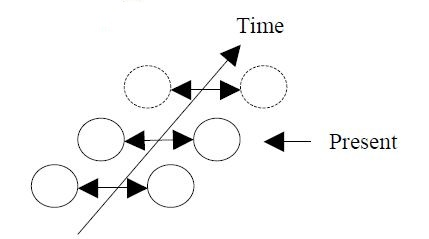
\includegraphics[scale=0.5]{interpersonal.jpg}
\caption{Eksisterende relasjon og avbrudd}
\label{interpersonal}
\end{figure}

\noindent
Avbrudd kan også ha effekter på andre mennesker som befinner seg på samme lokasjon som den som blir avbrutt. Dette illustreres i figur \ref{collateral}, hvor interaksjonen mellom aktør D (avbryter) og aktør B (den som avbrytes) også påvirker aktører A og C.
\begin{figure}[H]
\centering
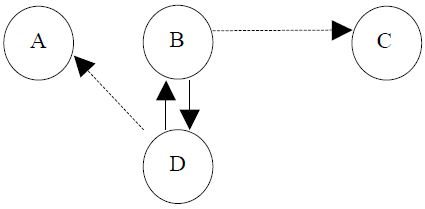
\includegraphics[scale=0.5]{collateral.jpg}
\caption{Lokasjonsbasert forstyrrelse}
\label{collateral}
\end{figure}

\noindent
En annen situasjon som kan oppstå er det Harr og Kaptelinin (2007) kaller frysing. Dersom aktører B og C utfører en oppgave ved synkron kommunikasjon, eksempelvis ansikt-til-ansikt eller per telefon, og aktør A avbryter aktør B, vil aktør C måtte vente til aktør B igjen blir tilgjengelig. 
\begin{figure}[H]
\centering
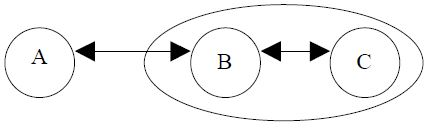
\includegraphics[scale=0.5]{frysing.jpg}
\caption{Frysing}
\label{frysing}
\end{figure}

\noindent
For en gruppe samarbeidende individer, vil oppgaver utført av et enkelt individ ofte være deler av den overordnete kollektive aktiviteten. Dermed vil forstyrrelsen av et individ sannsynligvis påvirke andre medlemmer i gruppen. Figur \ref{direkte} viser aktør B og aktør C som samarbeider om en gruppeoppgave GT, hvor GT er en del av den overordnete aktiviteten CA. Dersom aktør A avbryter aktør B, vil aktør C kanskje måtte dekke for aktør B, frem til B igjen blir tilgjengelig.
\begin{figure}[H]
\centering
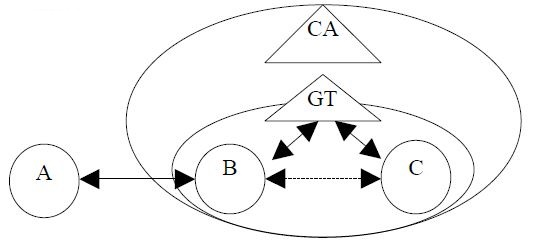
\includegraphics[scale=0.5]{coverme.jpg}
\caption{Samarbeid og avbrudd - direkte forstyrrelse}
\label{direkte}
\end{figure}

\noindent
Aktører B og C må ikke nødvendigvis kommunisere direkte, men aktør C kan være avhengig av tiden, innholdet og kvaliteten aktør Bs oppgave resulterer i. Dermed kan en forstyrrelse av aktør B også indirekte forstyrre aktør C.
\begin{figure}[H]
\centering
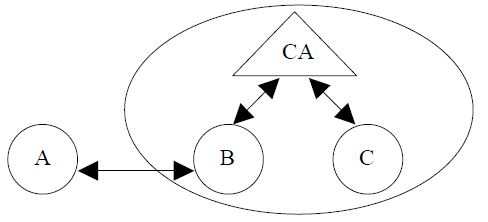
\includegraphics[scale=0.5]{dropball.jpg}
\caption{Samarbeid og avbrudd - indirekte forstyrrelse}
\label{indirekte}
\end{figure}

\noindent
Forskere som arbeider innen \emph{interruption value evaluation}-paradigmet tar utgangspunkt i at ikke alle avbrudd er dårlige, og at de ikke bør evalueres kun avhengig av hvordan de påvirker lokal kontekst, men også avhengig av hvor stor nytte de har. Målet er dermed å optimalisere individets beslutningstakingsprosess om hvordan han skal respondere på avbruddet. Den mest aktuelle teknikken for avbruddshåndtering vil derfor være forhåndsvisning av informasjon om avbruddet, hvem det er fra og hva det handler om, slik at individet selv kan reflektere over hvordan han/hun skal respondere basert på sin lokale kontekst. Dermed vil også det Grandhi og Jones (2010) kaller relasjonell kontekst være en del av avbruddskonteksten. Denne defineres som alle aspekter mellom den som avbryter og den som blir avbrutt, hvilken relasjon de har, hva avbruddet dreier seg om og deres tidligere interaksjonsmønstre.

\subsubsection{Utfordringer}
Harr og Kaptelinin (2007) påpeker tre fundamentale utfordringer ved avbruddshåndtering: (1) fare for å miste informasjon, (2) mindre privatliv og (3) utsettelse av oppgaver. For hver situasjon må individer finne den optimale balansen mellom isolasjon og tilgjengelighet, åpenhet og privatliv, og direkte eller utsatt håndtering av avbruddene.
\begingroup
\let\clearpage\relax
\section{Suksesskriterier ved implementering}
\label{chp: suksesskriterier}


\subsection{Brukbarhet}
\label{chp: brukbarhet}

Brukbarhet defineres i ISO 9241-11 \cite{Svanes08} som

\noindent
\begin{otherlanguage}{english}
\emph{the extent to which a product can be used by specified users to achieve specified goals with effectiveness, efficiency and satisfaction in a specified context of use.}
\end{otherlanguage}

\noindent
Brukbarhet er dermed et begrep som ikke kan måles generelt, men er relativt til bestemte brukere med bestemte mål i en spesifikk kontekst. Likevel kan man generelt definere noe som brukbart dersom det er funksjonelt, effektivt og tilfredsstillende \cite{Kuniavsky}. Et system er funksjonelt når det anses som nyttig av brukeren, og må dermed svare til de forventningene brukeren har til hva det skal gjøre, og faktisk gjøre det. Effektivitet kan måles som hvor raskt en er i stand til å utføre en oppgave med så lite feil som mulig. Det er vanskelig å konkretisere hva som gjør et system tilfredsstillende for en bruker, dette er individuelt og er en følelsesmessig respons ved bruk systemet \cite{Kuniavsky}. Ofte vil god design være avgjørende for om en bruker opplever systemet på en god måte, forutsett at det også er funksjonelt og effektivt. Designere av grensesnitt har gjennom årene kommet frem til en rekke reningslinjer for god design. Desverre er disse ofte blitt kritisert for å være både for spesifikke og ufullstendige \cite{mmi}. 
Interaktive applikasjoner og systemer vil spesielt hemmes av dårlig design dersom de allerede er vanskelige å lære og kompliserte å bruke. Slike systemer kan også føre til katastrofale utfall dersom kritisk informasjon ikke blir presentert på en effektiv måte. Det er derfor avgjørende å ha forståelse for hva slags informasjon brukeren trenger og hvordan denne skal presenteres \cite{Ebright10}. 

\subsubsection{Gestaltprinsippene}
Gestaltprinsippene har sitt navn fra det tyske \emph{gestalten}, som betyr "å forme". Prinsippene blir ofte referert til som lover, og det finnes mange varianter utviklet av forskjellige psykologer. Det de har til felles at de forklarer hvordan vi organiserer og tolker visuelle intrykk i områder og strukturer. Disse prinsippene beskriver blant annet virkningen av plassering av fokuspunkt, organisering av elementer, fargevalg, harmoni og enkelhet, og understeker at vi alle tolker visuelle inntrykk ut ifra egne erfaringer. 
Disse prinsippene ble i utgangspunktet brukt til å foreslå hvordan statiske visuelle elementer burde presenteres. I dag er det vanlig å ta hensyn til disse retningslinjene i design av blant annet skjermbilder \cite{Chang02}. 

\subsubsection{Affordance, konseptuelle modeller og begrensninger}
Vår forståelse av hvordan vi skal bruke en gjenstand første gang vi ser den beror på tre dimensjoner: konseptuell modell, begrensninger og \emph{affordance}. Ordet affordance ble innført av psykologen J. J. Gibson. Det finnes ingen norsk oversettelse, men begrepet refererer til hva slags handling en gjenstand signaliserer når du ser den for første gang \cite{Norman99}.

\noindent
Det skilles mellom ekte affordance og oppfattet affordance, hvor det først og fremst er oppfattet affordance vi kan kontrollere i skjermdesign. Ekte affordance vil med tanke på datamaskiner være tastatur, skjerm, knapper og musepeker som signaliserer handlinger som berøring, peking, trykking og å se på. Ekte affordance finnes alstå uavhengig av hva som vises på skjermen. Det som vises på skjermen er visuelle tilbakemeldinger som viser hva vi kan gjøre, altså oppfattet affordance \cite{Norman99}.

\noindent
Affordance blir ofte forvekslet med begrensninger og konvensjoner. Vi kan si å ha tre typer begrensninger:
\begin{enumerate}
\item Fysiske begrensninger, som har sammenheng med ekte affordance. Et eksempel på dette kan være at det er ikke mulig å flytte musepekeren utenfor skjermen. 
\item Logiske begrensninger er sterkt knyttet til en god konseptuell modell. Et eksempel på dette er hvordan brukeren vet at den må skrolle for å se resten av siden.
\item Kulturelle begrensninger er tillært og deles av en gruppe mennesker, eksempelvis hva det betyr når markøren skifter form.
\end{enumerate}
En konvensjon er en kulturell begrensning som har utviklet seg over tid, og som forbyr noe og oppfordrer til noe annet. Slike konvensjoner er langsomme, i den betydning at det tar lang tid før de blir adoptert, og når de først er blitt det, tar det vel så lang tid før de forsvinner \cite{Norman99}.

\noindent
Spesielt logiske og kulturelle begrensninger er sterke virkemidler innen skjermdesign, da designere er mer opptatt av hva brukerene oppfatter som mulig, fremfor hva som faktisk er sant. Tilbakemeldinger og reaksjoner fra skjermen hjelper oss å forstå hva vi kan og skal gjøre \cite{Norman99}.
\subsection{Utfordringer med CSCW}
\label{chp: utfordringerMedCSCW}

Mange CSCW-systemer faller til kort når det kommer til forventningene til deres suksess. Dette kommer gjerne til syne ved at de tiltenkte brukerene ganske enkelt unngår å bruke systemet, eller at de stadig må lage midlertidige løsninger (workarounds) for å få gejnnomført arbeidsoppgavene sine. Spesielt to grunner til dette er knyttet til kompleksiteten rundt å utvikle multibrukersystemer, som brukes samtidig av mange brukere på forskjellige nivåer og med forskjellige behov og perspektiver.

\noindent
For det første er det ofte manglede kunnskap om CSCW (multibruker-)systemer, i motsetning til enkeltbruker-systemer. En typisk CSCW-applikasjon eller system vil vanligvis bli brukt av et vidt spekter av forskjellige brukere, med forskjellig bakgrunn, erfaringer og forhold til bruk av informasjonssystemer generelt. Beslutningstakere, ofte ledere, vil ha en intuisjon for hva som vil være fordelaktige for brukere som en selv. Desverre kan de fort overse funksjoner som andre brukere vil ha nytte av, spesielt for fuksjoner som vil før til merarbeid for dem selv. 

\noindent
Det andre er at det vanskelig å lære fra tidligere feil, da CSCW-systemer er svært komplekse og unike for hvert enkelt tilfelle, noe som vanskeliggjør evaluering i ettertid. Det er også vanskelig, om ikke umulig å gjenskape miljøene og forholdene som er essensielle i den virekelige konteksten hvor et CSCW-system skal implementeres i et laboratorium. for ikke å snakke om utfordringene ved å gjøre feltobservasjoner, grunnet blandt annet variasjon i gruppesammensettning og miljømessige faktorer.


\subsection{Workarounds}
\label{chp: workarounds}

Workarounds defineres av Kobayashi (2005) som \emph{"informal temporary practices for handling exceptions to normal workflow"}. Direkte oversatt til norsk betyr det "å jobbe rundt", eller å finne midlertidige løsninger.
\noindent
Workarounds kan være nødvendig når det oppstår akutte situasjoner hvor man ikke har nødvendige ressurser tilgjengelig, eller de kan oppstå som følge av sperrer i et system. Disse sperrene kan være tilsiktede, eller utilsiktede. Et eksempel på førstnevnte finner vi i \cite{Vogelsmeier08}, hvor sykepleiere ikke kan bestille doser av medisiner høyere enn det som er anbefalt. I tilfeller hvor høyere doser likevel var skrevet ut av lege, bestilte pleierene bare flere doser. 
Et annet eksempel på en workaround er gitt av Klemets, Evjemo og Kristiansen (2013), som beskriver hvordan sykepleiere fordeler ansvar for pasienter når de skal gå til lunsj. I utgangspunktet fordeles ansvar for pasienter gjennom en bemanningsplan som konfigureres i en applikasjon kjørende på en PC i sengeområdet. Å endre på denne planen krever merarbeid, og noen sykepleiere velger derfor å ikke gjøre endringene, men heller gi muntlig beskjed til kolleger om at en går til lunsj. Dette fører til at telefonene ringer under lunsjpausen.

\noindent
Vogelsmeier (2008) beskriver workarounds som førstegrads problemløsing i den forstand at man lager mekanismer for å jobbe rundt problemer, uten å forsøke å løse den underliggende årsaken til at problemet oppsto.
Dersom workarounds oppstår som konsekvens av utilsiktede sperrer, eller der systemet er for rigid i forhold til sykepleierenes arbeidsmønster slik at systemet ikke støtter opp om arbeidet på en tilfredstillende måte, er dette svært uheldig. Dette kan i verste fall føre til livstruende situasjoner.
Selv om slike workarounds er vanlige i medisinske settinger, er de som beskrevet ikke nødvendigvis effektive og vellykkede. Workarounds som gir organisatoriske løsninger for unntak som stadig gjentar seg, og dermed reduserer den kognitive innsatsen som kreves for å håndtere nye krisesituasjoner, vil ofte være suksessfulle. Workarounds som derimot gir ringvirkninger av ustabilitet i resten av organisasjonen, kan sies å være lite suksessfulle, selv om de løser problemet der og da \cite{Kobayashi05}.
\subsection{Motstand mot endring}
\label{chp: motstand}

Implementering av nye informasjonssystemer kan by på utfordringer for ledelsen og utviklere dersom de ansatte viser motstand mot endringen. 
En slik endring vil påvirke menneskene som jobber der, deres sosiale relasjoner og forholdet mellom mennesker i og utenfor organisasjonen. Derfor kan det oppstå motstand uavhengig av hvor godt systemet som implementeres er, og i hvor stor grad de ansatte har fått bidra i utviklingen i form av medvirkning \cite{Jacobsen12}. Cavaye (1995) kaller denne motstanden for mellomliggende variabler, og understreker at sli
orhold til designer/utvikler og deres innspill blir hørt. Det finnes flere årsaker til slik motstand mot endring, og vi vil her forklare noen av dem. 

\subsubsection{Faglig uenighet}
De ansatte kan være faglig uenige i selve endringen. Verken analyser av dagens situasjon, behovet for endring eller selve endringen er klare og objektive størrelser, og det er derfor også rom for uenigheter rundt det faktiske behovet for endring, og hvorvidt endringen som gjennomføres er den rette løsningen på problemet. \cite{Jacobsen12}

\subsubsection{Merarbeid}
En endring i seg selv kan kreve ekstraarbeid fra de ansatte, spesielt i en overgangsfase. Det kan være mye nytt å sette seg inn i og lære, noe som krever en ekstra innsats, ofte uten tilstrekkelig kompensasjon, noe mange stiller seg negative til. Slikt ekstraarbeid kan i tillegg til å lære noe nytt innebære at man må avlære de gamle måtene å jobbe på. \cite{Jacobsen12}

\subsubsection{Systemet som en trussel}
Dersom brukerene ser på det nye systemet som en trussel mot deres nåværende kontroll over eget arbeid, eller deres posisjon i form av deres ekspertise, vil de mest sannsynlig motsette seg endringen det nye systement representerer. \cite{Cavaye95}

\subsubsection{Grad av medvirkning}
Motstand kan også oppstå dersom det faktiske nivået av medvirkning avviker fra det nivået brukeren ønsker seg. Dette gjelder ikke bare dersom nivået er lavere, men også dersom nivået av medvirkning blir høyere enn det brukeren så for seg i utgangspunktet. Det er derfor ikke tilstrekkelig med medvirkning i seg selv, den må også møte brukerenes forventninger. \cite{Cavaye95}

\noindent
Jacobsen(2012) hevder at indre motivasjon og involvering de ansatte, slik at de føler seg som medeiere i endringsprosessen er avgjørende for å få de ansatte motivert for endringen og dermed redusere overnevnte motstand. Bred deltagelse på denne måten gir den enkelte ansatte opplevelsen av at den er med på å forme sin egen fremtid, og at dette vil skape en aksept og forståelse for usikkerheten som er assosiert med en hver endring.
\subsection{Brukermedvirkning og deltagende design}
\label{chp: medvirkning}

\subsubsection{Brukermedvirkning}
Uttrykket \emph{brukermedvirkning} er sammensatt av to aspekter, \emph{bruker} og \emph{medvirkning}. For å forstå hva brukermedvirkning egentlig er må vi forstå de to aspektene enkeltvis. Vi må anerkjenne at det finnes flere typer \emph{brukere}. Det kan være toppledelsen, som bruker systemets output i sine analyser og strategiske avgjørelser. Det kan være mellomledere som er ansvarlig for, og overvåker, avdelinger som bruker systemet. Til sist har vi de ansatte som bruker systemet i sitt daglige arbeid. Det er ofte naturlig at alle brukergruppene tar del i utviklingsprosessen i større eller mindre grad. Toppledelsen må kanskje godkjenne systemet, og kan ha meninger om hva slags rapporter det skal generere. Mellomledelsen og andre ansatte kan bidra med innsikt i dagens arbeidsrutiner, problemer og workarounds, samt kravspesifikasjoner, ønsker til design og testing. Vi må også forstå at \emph{medvirkning} ikke er det samme som involvering, selv om de to uttrykkene ofte blir brukt om hverandre. I Cavaye (1995) finner vi definisjonene av (bruker)medvirkning og involvering som henholdsvis \emph{"a set of operations and activities performed by users"} i løpet av utviklingsprosessen, og \emph{"subjective psycological state"} som påvirker brukernes forestillinger, og dermed systemets grad av suksess.

\noindent
Brukermedvirkning finner vi i mange former og på flere nivåer. Som vi ser i tabell \ref{Beskrivelse av brukermedvirkning} kan medvirkning beskrives ved hjelp av flere attributter. 

\begin{table}[H]
\caption{Beskrivelse av brukermedvikrning (hentet fra Cavaye (1995))}
%\centering
\begin{tabular}{c c}
\hline\hline
\textbf{Medvirkningsattributter} & \textbf{Mulige verdier} \\ [2ex]
\hline
& alle brukere \\[-1ex]
\raisebox{1.5ex}{Type} & representativt utvalg av brukere \\ [2ex]
\hline
& rådgivende \\ & signeringsansvar  \\
\raisebox{2ex}{Grad} & del av teamet \\ & fullt ansvar \\ [2ex]
\hline
& teknisk design \\
\raisebox{1.5ex}{Innhold} & sosialt og teknisk design \\ [2ex]
\hline
& prosjektdefinering  \\ & kravspesifikasjon  \\
\raisebox{2ex}{Område} & utvikling \\ & testing \\ [2ex]
\hline
& formell \\
\raisebox{1.5ex}{Formalitet} & uformell \\ [2ex]
\hline
& innspill ignorert \\
\raisebox{2ex}{Innflytelse} & bidrag tatt i betraktning  \\ & innspill tas seriøst \\
\hline
\end{tabular}
\label{Beskrivelse av brukermedvirkning}
\end{table}

\begin{itemize}
\item Type medvirkning beskriver andelen av brukere som faktisk blir inkudert. Det er ikke alltid det lar seg gjøre å inkludere alle brukere i praksis. Da er det viktig å etterstrebe å ha et representativt utvalg av disse med i prosessen.
\item Grad av medvirkning viser til at brukere har forskjellig grad av ansvar gjennon sin medvirkning.
\item Innholdet i medvirkningen refererer til det faktum at brukerne kan involveres i forskjellige aspekter av utviklingsprosessen. Det er vanlig at brukere involveres i aktiviteter som forbereder det tekniske designet av systemet, men de kan også involveres i det sosiale designet, det vil si de menneskelige og sosiale effektene systemet vil ha.
\item Området medvirkningen angår vil variere gjennom de forskjellige fasene av utviklingsprosessen. Medvirkning fra brukerne er mer vanlig i forbindelse med å sette rammer for prosjektet, kravsspesifikasjon og testing enn gjennom selve utviklingen og kodingen av systemet.
\item Medvirkningen kan være formell, ved bruk av formelle grupper og team, eller uformell, med tilfeldige diskusjoner og oppgaver.
\item Innflytelsen brukerene faktisk har kan variere, og innspill fra disse kan vektlegges i forskjellig grad av utviklerene, alt fra å bli totalt ignorert til å bli tatt svært seriøst. Dette betyr at det kan legges ned mye ressurser i å la brukerne få komme med innspill, men at virkningen av disse beror på i hvilken grad disse blir tatt hensyn til.
\end{itemize}

\noindent
I mange år ble det sett som en selvfølge at brukermedvirkning hadde en signinfikant positiv effekt på en eventuell suksess for et informsjonsystem. Empiriske studier kan imidlertid ikke bevise at det alltid er en slik sammenheng \cite{Cavaye95}. Dermed ser det ut til at brukermedvirkning hverken er tilstrekkelig eller ytterst nødvendig for å garantere suksess for et informasjonsystem. 
Det er flere grunner til dette, sett fra både designers/utviklers og brukerens side. For det første har forholdet mellom bruker og designer/utvikler stor innvirkning på effekten av medvirkningen. Forskjeller i bakgrunn, erfaring og perspektiver kan føre til konflikter som igjen preger effekten av medvirkningen på en negativ måte. For det andre spiller det ingen rolle i hvor stor grad brukerne medvirker i prosessen dersom deres innspill blir ignorert. For det tredje vil de ansattes motstand mot endring kunne resultere i ubrukte systemer, eller bevisst sabotasje av implementeringen og endringsprosessen. Som beskrevet i avsnitt \ref{chp: motstand}, vil motstand mot endring kunne reduseres ved god informasjon og involvering (til forskjell fra medvirkning) av de ansatte. Dette må ikke sees som en motsetning til Cavaye (1995)s påstand om at medvirkning ikke er en garanti for suksess. Dette fordi informasjon til og involvering av de ansatte ikke nødvendigvis behøver å inkludere medvirkning, og fordi selv med medvirkning og innspill fra de ansatte er en ikke garantert å redusere motstanden tilstrekkelig til å sikre en suksessfull implementering av det nye systemet \cite{Cavaye95}.

\subsubsection{Deltagende design}
\label{dd}
Deltagende design er én av mange teknikker for å oppnå brukermedvikning.
Interessen for denne teknikken blir stadig større, og sees på som en god måte å blant annet sikre gode innspill fra brukere (for blant annet analyse av dagens situasjon), gjensidig læring og bedring av arbeidsrutiner.

\noindent
Vi kan dele utvikling av informasjonsystemer i tre aspekter: analyse, design og praksis. Det kan være vanskelig å kombinere alle tre samtidig, og tidligere ble det sett på som svært positivt om man greide å kombinere to av disse. Mogensen og Trigg (1992) ser i sin studie på muligheten for å kombinere alle tre aspektene samtidig (figur \ref{Challenge_PD}).

\begin{figure}[H]
\centering
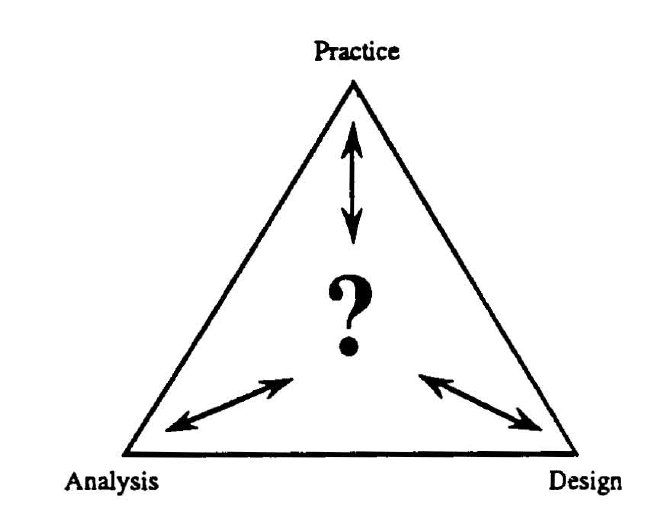
\includegraphics[scale=0.3]{Challenge_PD.jpg}
\caption{Hvordan kombinere alle?}
\label{Challenge_PD}
\end{figure}

\noindent
Ifølge \cite{Mogensen92} er det flere måter å oppnå større medvirkning på. Én teknikk er \emph{fremtidsworkshops}, der en ønsker diskusjon rundt mulige fremtidige løsninger på nåværende problemer, identifisert av brukerne selv. En annen teknikk er workshops hvor en bruker mock-ups og prototyper for å trigge diskusjon om mulige fremtidige teknologier og løsninger. Uavhengig av valgt teknikk vil graden av relevans til dagens praksis være avgjørende for workshopens suksess. Felles for de to er at de tar i bruk kontekstuelle artefakter (artefakter medbrakt av fasilitator som brukerene selv setter i kontekst).

\noindent
Mogensen og Trigg (1992) konkluderer med at bruk av kontekstuelle artefakter og hvor alle de tre faktorene, analyse, praksis og design er tilstede kan lede til nettopp et slikt ønsket samspill som vist i figur \ref{Artifacts_PD}. De argumenterer for at bruk av artefakter under en workshop ikke bare gir innspill på design - deltagende design, men at de også kan trigge diskusjoner som gir utviklerene bedre innsyn i dagens praksis, problemer og workarounds - deltagende analyse. 

\noindent
Deltagende design på denne måten, med bruk av kontekstuelle artefakter, gir derfor forskere/utviklere en dypere forståelse av hva som er problemområdene, og hvordan brukerne selv oppfatter dagens situasjon. Det gir også brukerne mulighet til større bevissthet rundt egne arbeidsmetoder, -rutiner og workarounds.

\begin{figure}[H]
\centering
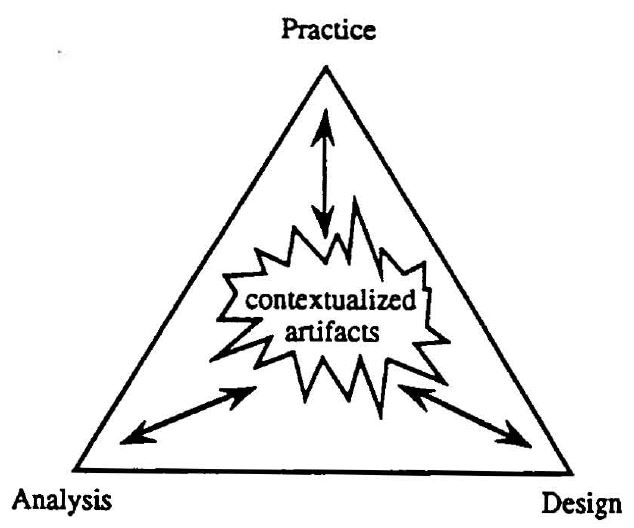
\includegraphics[scale=0.3]{Artifacts_PD.jpg}
\caption{Kontekstuelle artefakter støtter samspillet mellom de tre perspektivene}
\label{Artifacts_PD}
\end{figure}
\endgroup
\chapter{Forskningsmetode og hensikt}
\label{chp:forskningsmetode}

“I just want to develop a computer-based system” (Oates, 2006)

\noindent
Ifølge Oates (2006) er design og utvikling av ethvert databasert produkt en form for forskning som krever innsamling av data, analyse og konklusjon. For å utvikle et produkt eller system som skal utføre gitte oppgaver er det viktig å besvare hva disse oppgavene er, og hvorfor de er viktige. Dette besvares ved å samle informasjon om hva man ønsker av systemet, generere egen data som dokumenterer hvordan og hvorfor man designer og implementerer produktet, og deretter brukerteste og evaluere det. Vi vil i dette kapittelet først presentere hensikten med prosjektet før vi går i detalj på hvilke tilnærminger og metoder vi har valgt for å besvare forskningsspørsmålene.


\begingroup
\let\clearpage\relax
\section{Hensikt}
\label{chp: hensikt}

Hensikten gjenspeiler den underliggende grunnen til å gjøre forskning, hva som gjør den interessant og hvorfor den er viktig eller nyttig. Videre kan man se på hvorfor man ønsker å forske på noe \cite{Oates}. 

\noindent
Motivasjonen for oppgaven var innledningsvis å avdekke fordeler og utfordringer i det eksisterende pasientsignalsystemet, og hvordan det kunne videreutvikles for å bedre støtte sykepleierenes behov. En gjennomgang av tidligere arbeid ga en bredere forståelse av forskningsområdet, og vi ønsket derfor å utdype problemstillingen. Vi formulerte to forskningsspørsmål som søkte svar på hvorvidt informasjon om kollegers aktiviteter og tilgjengelighet er nyttig, og hvordan slik informasjon kan kommuniseres på en hensiktsmessig måte. Da tidligere arbeid viste at avbrytelser kan ha en negativ effekt på sykepleieres arbeid, ønsket vi samtidig å undersøke hvordan systemet kan endres for å redusere eventuelle negative effekter.

\subsubsection{Forskningsspørsmål}
Vi har formulert to spørsmål som vi søker svar på gjennom denne oppgaven. Disse er som følger:

\begin{enumerate}
\item Er informasjon om kollegers aktiviteter og tilgjengelighet nyttig for sykepleiere, og hvordan kan slik informasjon distribueres på en hensiktsmessig måte? 
\item Hvordan kan systemet endres for å begrense potensielle negative effekter ved avbrytelser?
\end{enumerate}

\section{Prosess}
\label{chp: prosess}

Prosessen i et forskningsprosjekt kan beskrives som sekvensen av aktiviteter som utføres i løpet av prosjektets varighet \cite{Oates}. Vi vil nå gjøre rede for de metodene og tilnærmingene vi har valgt i vår prosess.

\subsection{Paradigme}
Et paradigme er et sett felles antakelser om, eller måter å tenke på, noen aspekter av verden \cite{Oates}. Innen samfunnsforskningen fremstår kvalitativ og kvantitativ forskning som to vesentlige tenkemåter, eller paradigmer, når det gjelder hvordan man kan framskaffe eller generere informasjon om samfunnet, for deretter å analysere det (Tjora, 2010).
[SKRIV OM KVALITATIV vs KVANTITATIV, INDUKTIV, DEDUKTIV OG ABDUKTIV]

\subsection{Litteraturstudie}
Teorien vi har lagt frem i kapittel \ref{chp:teori} er basert på et litteraturstudie gjort innledningsvis i arbeidet. For å definere forskningsspørsmålene knyttet til oppgaven, analyserte vi i første omgang tidligere arbeid gjort av Klemets, Evjemo og Kristiansen (2013). Dette ga oss et inntrykk av forskningsområdet og utfordringene knyttet til det eksisterende pasientsignalsystemet. 

\subsection{Dokumentstudie}

\subsection{Prototype}
Ifølge Schneiderman og Plaisant (2010) mislykkes mange utviklingsprosjekter i å nå sine mål, i stor grad grunnet dårlig kommunikasjon mellom utviklere og brukere. Suksessfulle utviklere legger derfor stor vekt på å forstå kundens behov og krav. 
Brukersentrert design gir systemer som genererer færre problemer under utviklingen, og lavere vedlikeholdskostnader. De er enklere å lære, gir raskere ytelse og vesentlig mindre feil \cite{mmi}.
Prototyping er en velkjent måte å utforske og uttrykke design for interaktive systemer. 

\tikzstyle{mybox} = [draw=black, fill=white, very thick,
    rectangle, inner sep=10pt, inner ysep=20pt, rounded corners]
\tikzstyle{fancytitle} =[fill=black, text=white]
\begin{tikzpicture}
\node [mybox] (box){%
    \begin{minipage}{0.9\textwidth}
      En prototype defineres som enhver representasjon av en designidé, uavhengig av medium \cite{Houde97}.
    \end{minipage}
};
\node[fancytitle, rounded corners, right=10pt] at (box.north west) {Definisjon av prototype};
\end{tikzpicture}%



\subsection{Workshop}
\label{subsec:workshops}

Tjora (2012) påpeker at valg av metode for datagenerering må reflektere hva man faktisk ønsker å finne ut, og at effektivitet bør vektlegges. “Datagenereringen må kunne frambringe mest mulig relevant og pålitelig informasjon uten unødig bruk av forskeres og deltageres tid og ressurser”.
I tråd med \ref{chp: medvirkning}, ønsket vi en brukersentrert designprosess, hvor brukerene medvirket gjennom en \emph{deltagende design workshop}.
En slik workshop åpner for at utviklere, bedriftsrepresentanter og brukere kan jobbe sammen for å avdekke utfordringer og løsninger på en svært produktiv måte. Dette vil være mest effektivt tidlig i designprosessen, da idèer ikke hemmes av eksisterende kode eller annen infrastruktur \cite{Gaffney99}.

\subsubsection{Kontekst}
Vi gjennomførte to workshoper over to dager. Disse ble holdt på NSEP brukbarhetslab (Norsk senter for elektronisk pasientjournal) ved St. Olavs Hospital. Brukbarhetslaben er bygget for å kunne observere og teste mobile helsetjenester \cite{NSEP}.
Som Alsos og Dahl (2008) beskriver, vil sykehus ofte ha strenge restriksjoner mot å tillate eksperimentelle forsøk, da slike forsøk kan ha en påtrengende effekt på det pågående arbeidet. I tillegg kan opptak av observasjoner være forbudt, da pasientinformasjon er konfidensielt. Ved testing i brukbarhetslab kan man fokusere på relevante bruksområder og kontrollere faktorer irrelevante for evaluering av løsningen \cite{Alsos08}. På grunn av tidsbegrensning var det derfor naturlig å benytte brukbarhetslaben som testmiljø.   

\noindent
Alsos og Dahl (2008) påpeker at det er viktig at de fysiske testomgivelsene, testscenarioene og prototypene er så realistiske som mulig for å kunne generere gyldige resultater. Da workshopene ble arrangert på NSEP hvor det eksisterende pasientsignalsystemet ikke er implementert, valgte vi å lage mock-ups av paneler og telefoner, se figur \ref{systemmockup} og \ref{mock-up_VaktPanel}. Vi brukte to pasientrom, med en gang i mellom, for å etterligne sengetunet. Ved å gjøre de fysiske omgivelsene mer realistiske, kunne vi i større grad studere gjeldende arbeidspraksis.

\begin{figure}[H]
	\centering
	\begin{subfigure}[b]{0.25\textwidth}
		\centering
		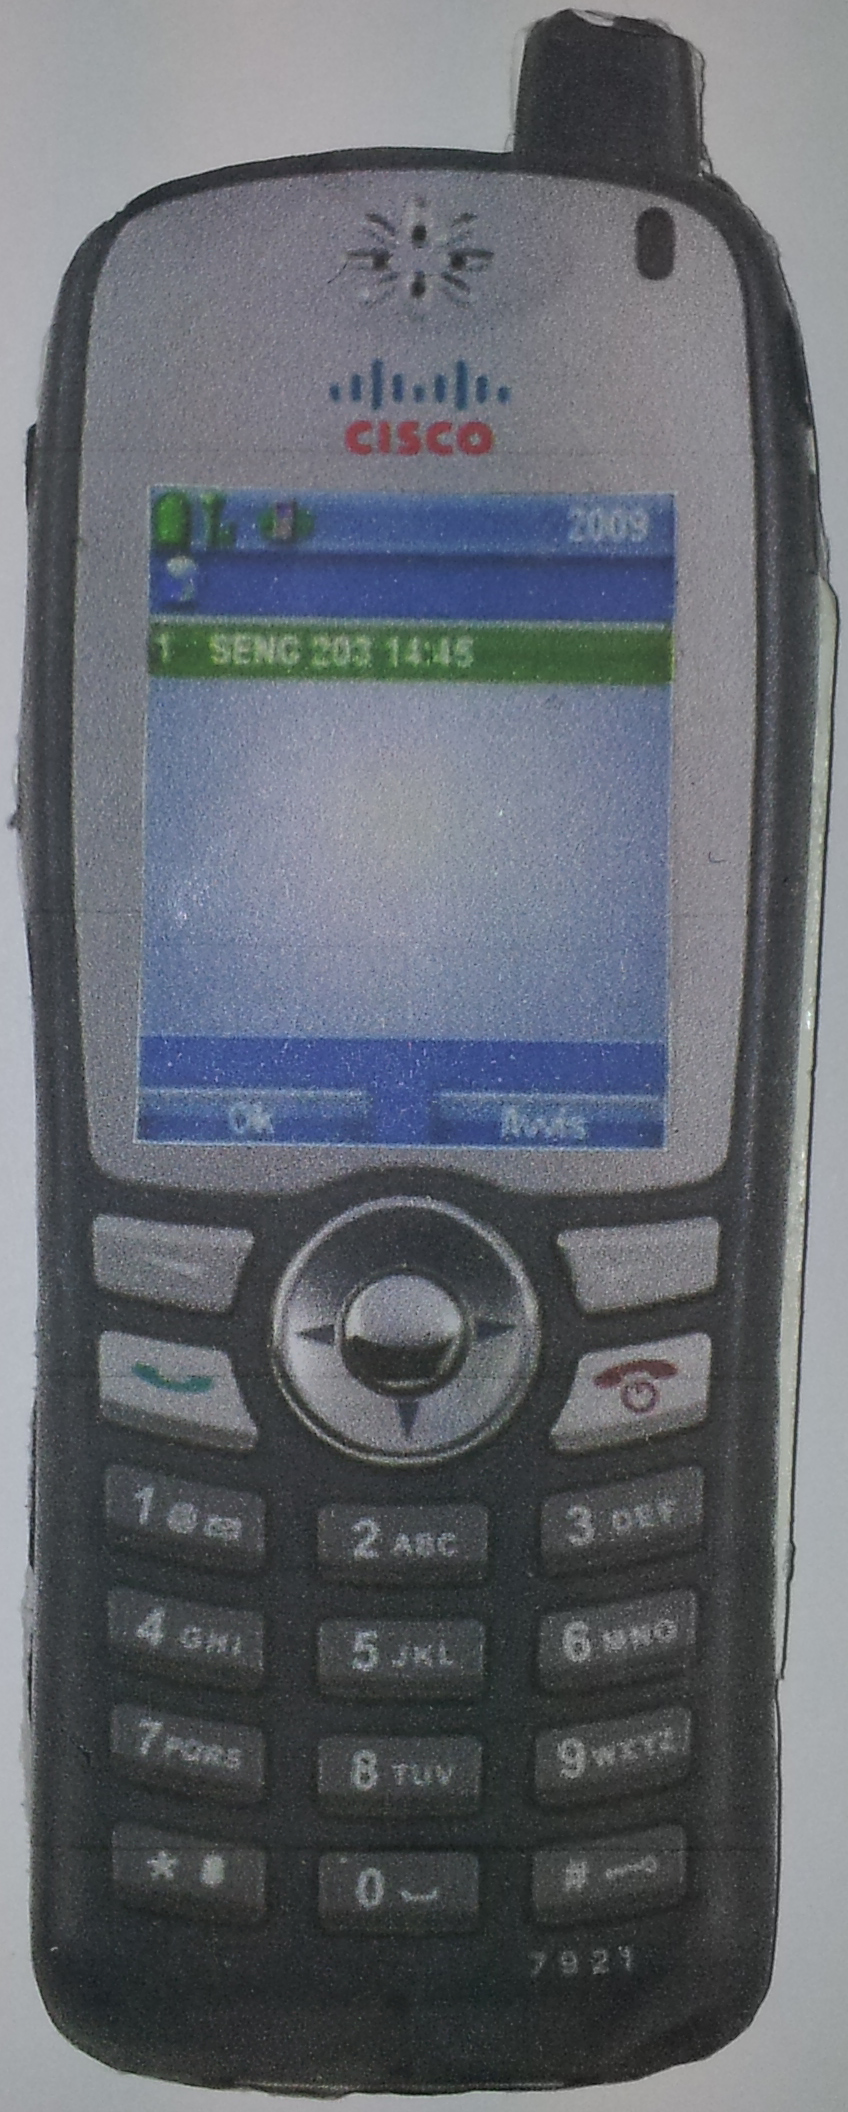
\includegraphics[scale=0.07]{mock-up_Telefon.jpg}
		\caption{Mock-up av telefon}
		\label{mock-up_Telefon}
	\end{subfigure}
	\begin{subfigure}[b]{0.35\textwidth}
		\centering
		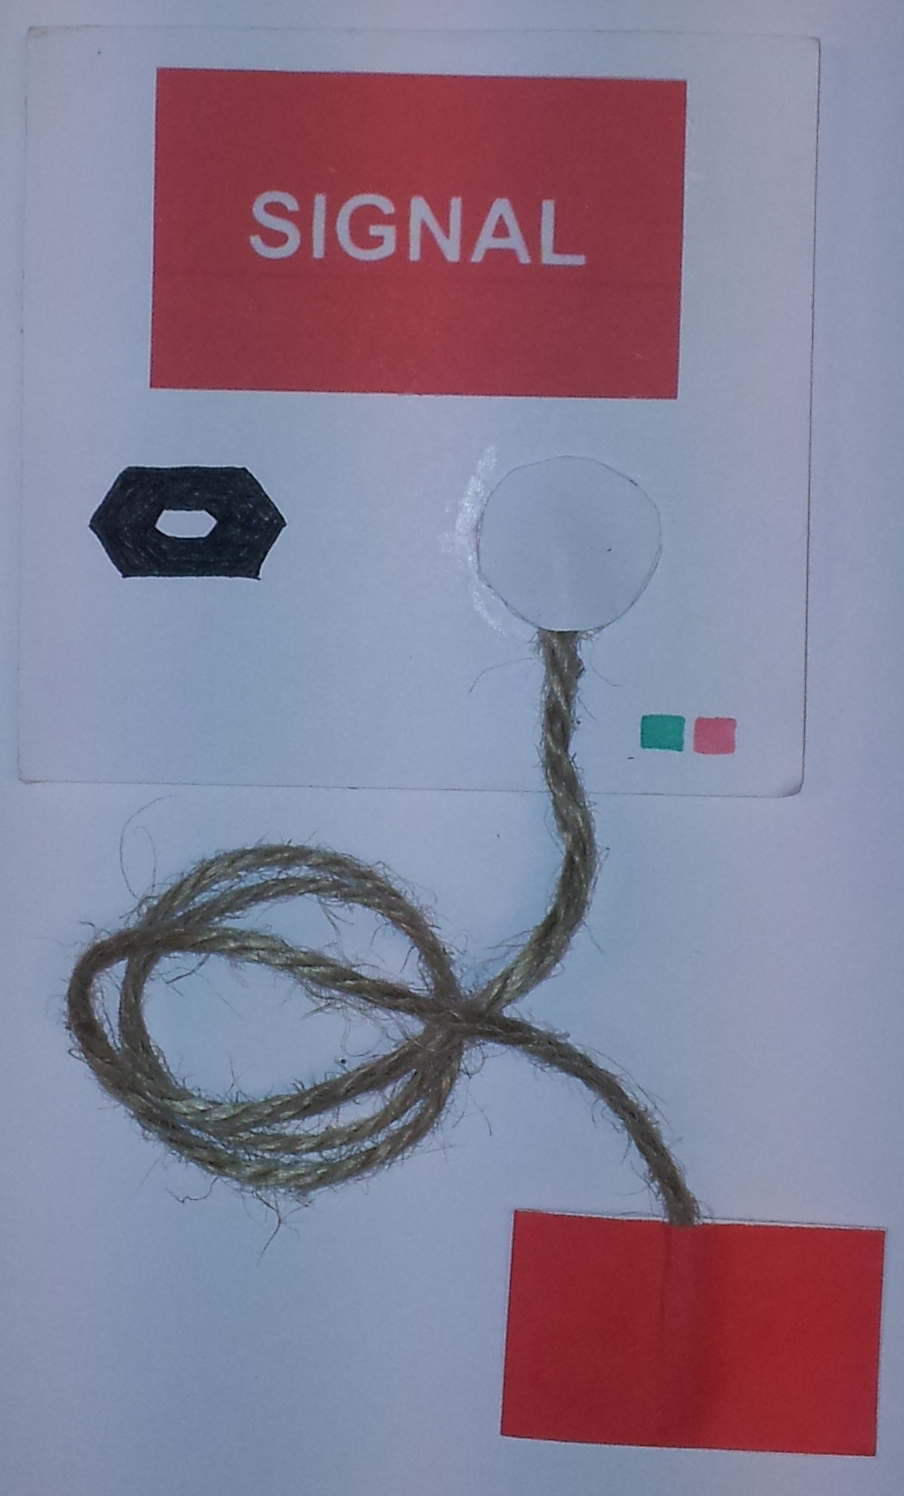
\includegraphics[scale=0.07]{mock-up_PasientPanel.jpg}
		\caption{Mock-up av anropspanelet}
		\label{mock-up_PasientPanel}
	\end{subfigure}
	\begin{subfigure}[b]{0.35\textwidth}
		\centering
		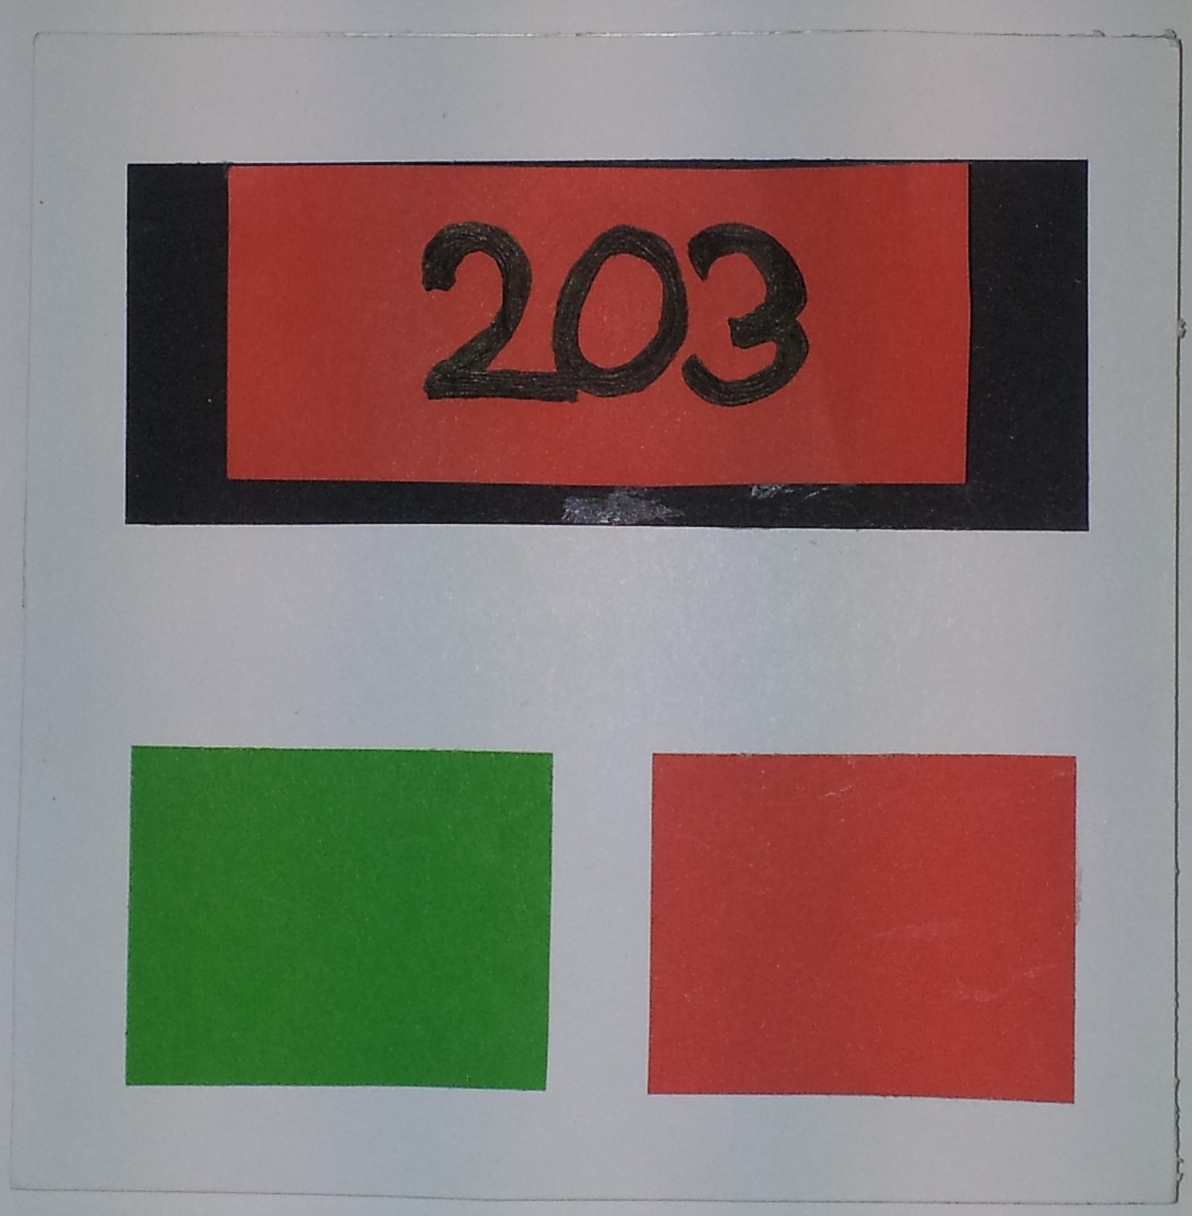
\includegraphics[scale=0.07]{mock-up_RomPanel.jpg}
		\caption{Mock-up av rompanelet}
		\label{mock-up_RomPanel}
	\end{subfigure}
	\caption{Mock-up av pasientsignalsystemet}
	\label{systemmockup}
\end{figure}

\begin{figure}[H]
\centering
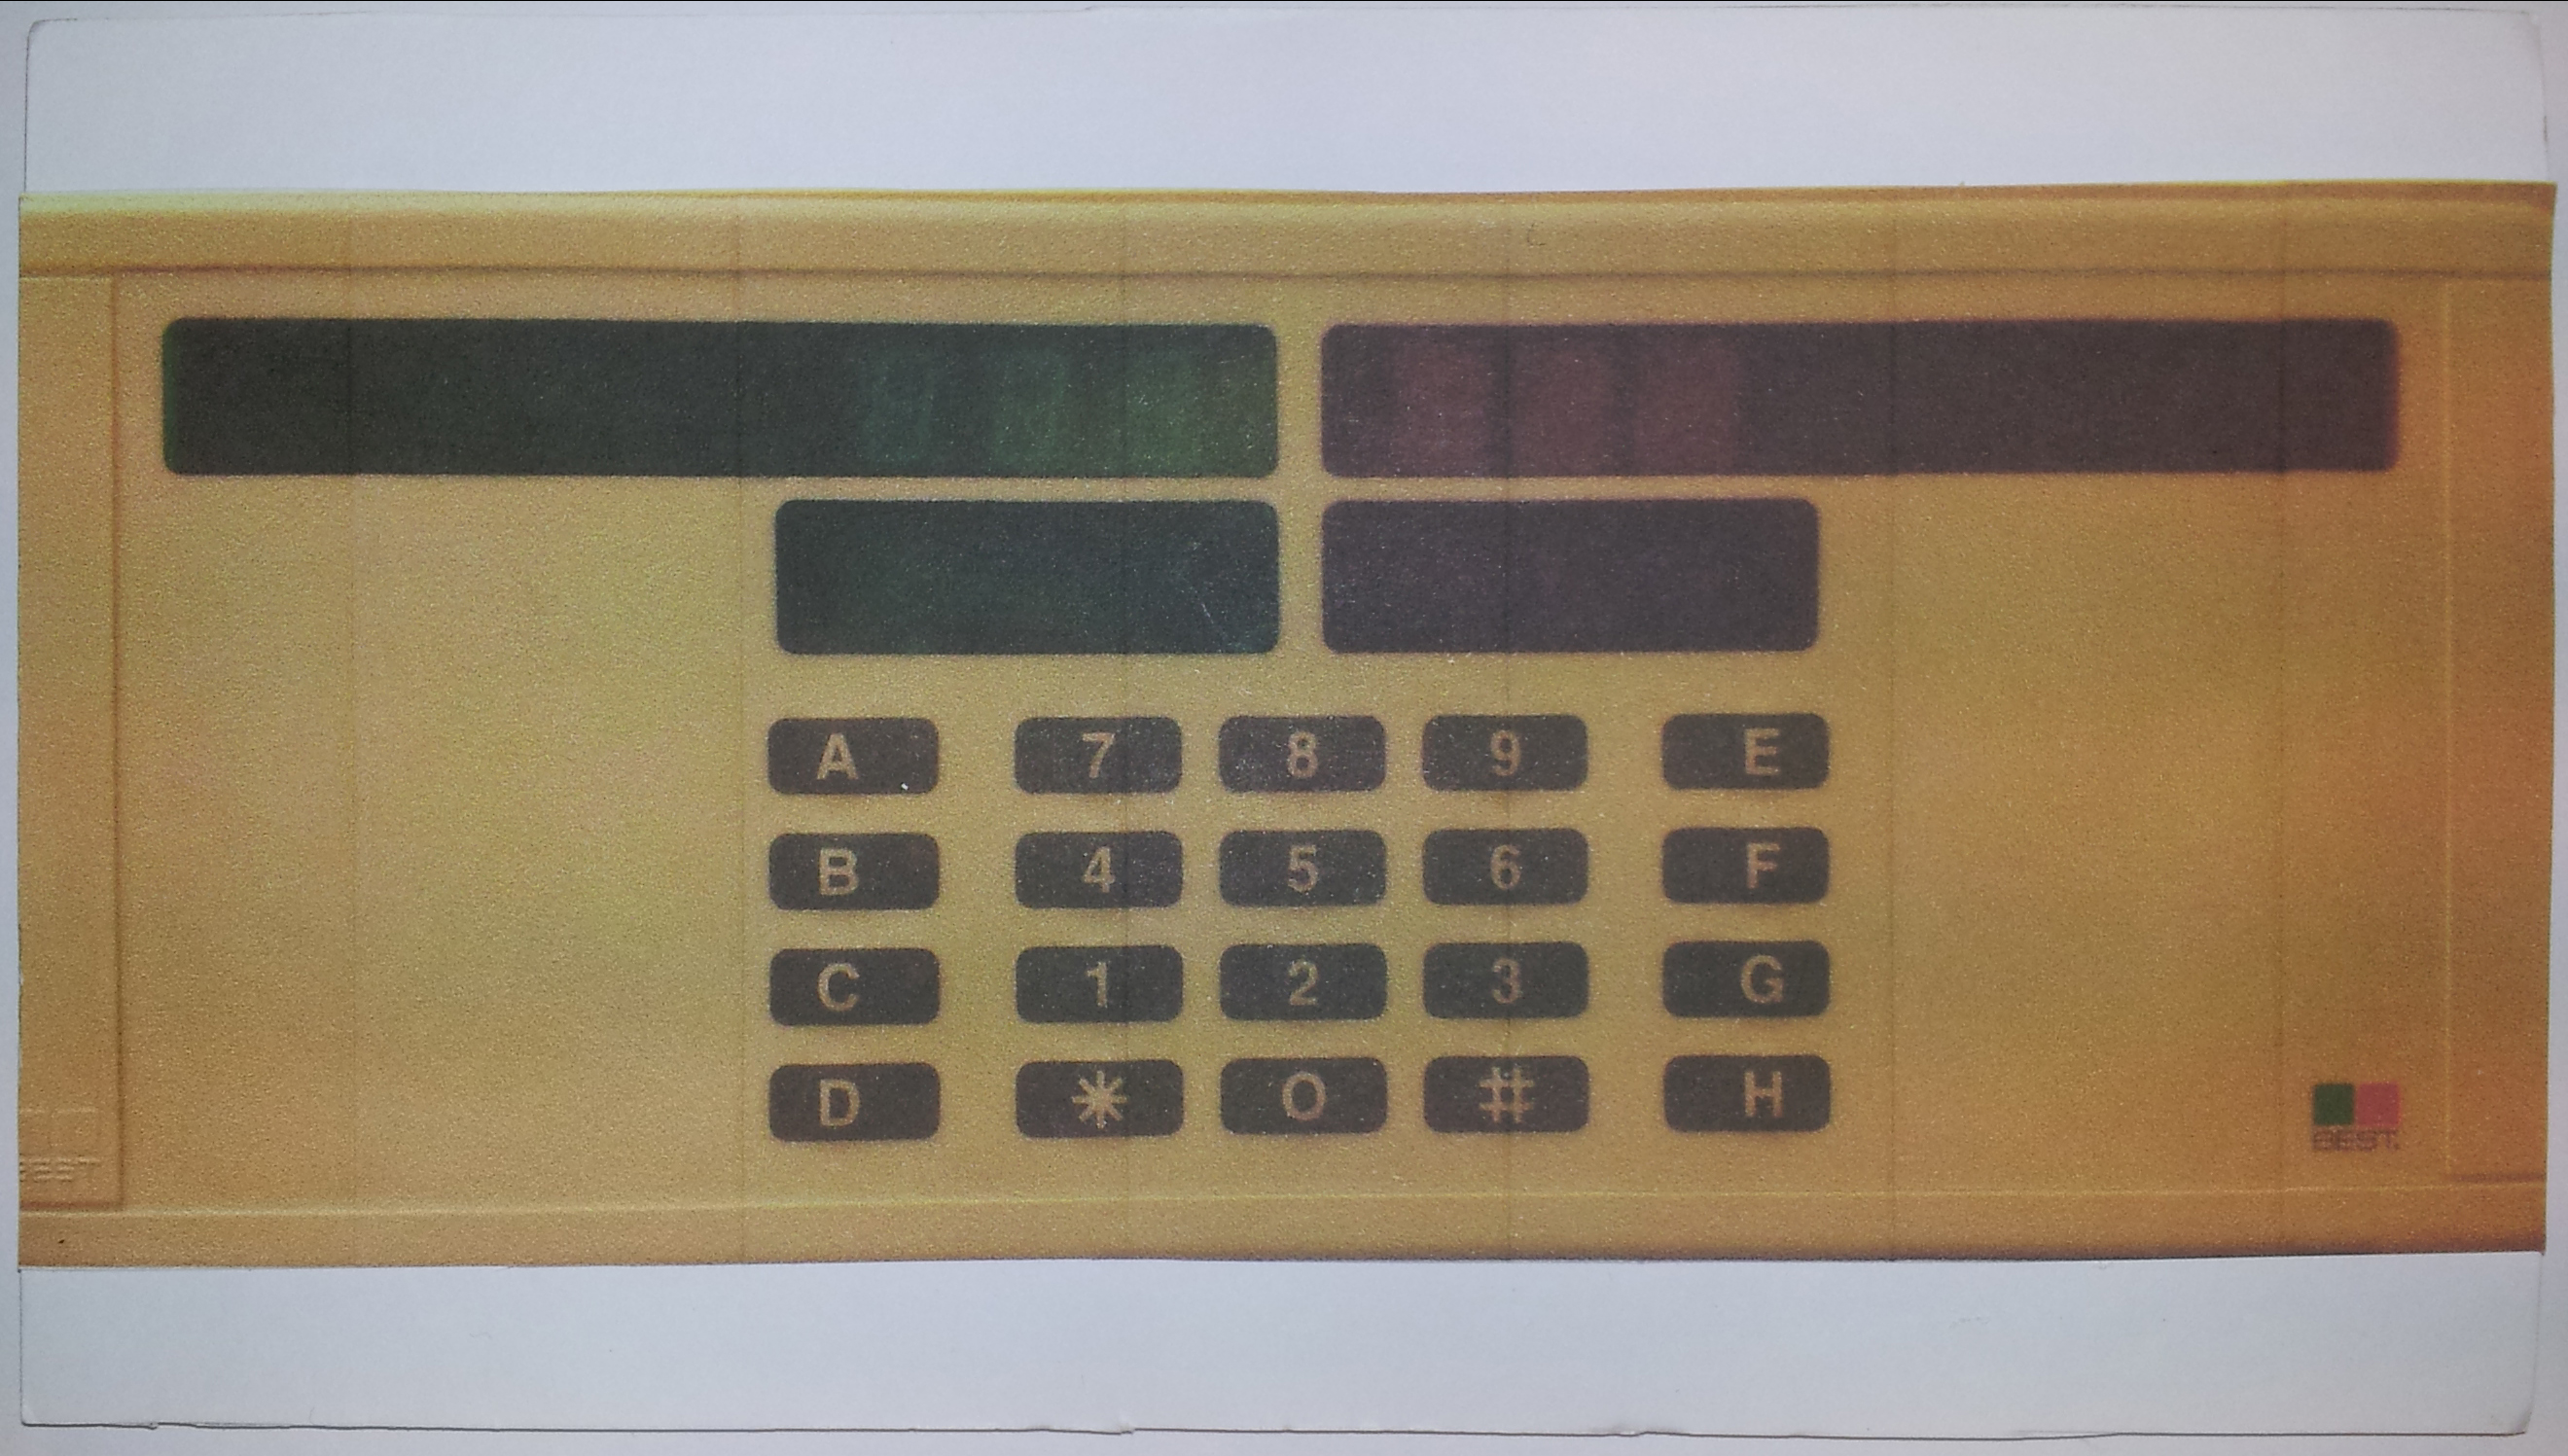
\includegraphics[scale=0.07]{mock-up_VaktPanel.jpg}
\caption{Mock-up av vaktromsapparatet}
\label{mock-up_VaktPanel}
\end{figure}

\subsubsection{Scenarioer}
Som beskrevet av Svanæs og Seland (2004), er rollespill med bruk av lavnivå-protoype en god måte å få brukere og utviklere "opp av stolen", og gjør det mulig å utforske designkonsepter med brukere i en tidlig fase. Scenario-basert design, belyst av Bardram (2000), er nyttig i situasjoner hvor man ikke har en detaljert oppfattelse av nøyaktig hvilke arbeidsaktiviteter som skal støttes, og på hvilken måte. Denne designprosessen har to karakteristikker, (1) man ønsker å re-designe de eksisterende måtene å gjøre ting på for å forstå hvordan ting kan gjøres annerledes ved hjelp av et datasystem. Dette starter ofte ved at man undersøker problemene og fordelene med det eksisterende systemet. (2) Deretter starter den kreative prosessen, hvor designeren, med sin tekniske erfaring, og brukeren, med sin arbeids- og organisasjonserfaring, sammen kommer opp med nye ideer. Relevante spørsmål man bør stille seg i en slik prosess er; er disse ideene nyttige? Og hvilke arbeidsaktiviteter støtter de, og hvilke forstyrrer de? Bruk av scenarioer er dermed nyttig fordi de støtter det kreative samspillet mellom designer og bruker, og de besvarer spørsmål om nyttigheten til systemet i forhold til arbeidsrutinene i en organisasjon. Arbeidsaktivitets-scenarioer, er scenarioer som prøver å få en klarhet i det arbeidet vi ønsker å designe for. 
I tråd med det Bardram (2000) skriver, var det ønskelig å bruke to sett med scenarioer, ett hvor det eksisterende systemet og arbeidspraksis ble brukt, og ett hvor vi testet våre ideer i form av en prototype, for å skape en kreativ prosess for videre forslag og innspill fra deltagerne. Det ble tatt utgangspunkt i scenarioer og pasientbeskrivelser fra Selseth (2012)\nocite{Selseth12}, med noen modifikasjoner for å gjøre de relevante til våre forskningsspørsmål. Scenarioene i sin helhet er vedlagt som en del av tillegg B, og pasientbeskrivelsene er vedlagt i tillegg C.

\noindent
Rollen som fasilitator 

%\begin{adjustbox}{with=\textwith, hight=\texthight}
\begin{table}[H]
%\small
%\centering
\begin{tabular}{l|l|l|l|l}
\hline
\textbf{\begin{tabular}[x]{@{}c@{}}Del av\\workshop\end{tabular}} & \textbf{Beskrivelse} & \textbf{Hvor} & \textbf{Tidspunkt} & \textbf{Varighet}\\
\hline
Steg 1 & Informasjon & \begin{tabular}[x]{@{}c@{}}Rundt bord\\/i gangen\end{tabular} & 13:00-13:15 & 15min\\
\hline
Steg 2 & Fokusgruppe med scenarioer & \begin{tabular}[x]{@{}c@{}}Rundt bord\\/i gangen\end{tabular} & 13:15-13:45 & 30min\\
\hline
& \textbf{Pause} & & 13:45-13.50 & 5min\\
\hline
Steg 3 &\begin{tabular}[x]{@{}c@{}} Scenarioer med rollespill\\- uten prototype\end{tabular} & Inne på sengerom & 13:50-14:25 & 35min\\
\hline
Steg 4 &\begin{tabular}[x]{@{}c@{}}Scenarioer med rollespill\\- med prototype\end{tabular} & Inne på sengerom & 14:25-15:00 & 35min\\
\hline
& \textbf{Pause} & & 15:00-15:15 & 15min\\
\hline
Steg 5 & Fokusgruppe/oppsummering & \begin{tabular}[x]{@{}c@{}}Rundt bord\\/i gangen\end{tabular} & 15:15-16:00 & 45min
\end{tabular}
\label{Plan}
\caption{Overordnet plan for dagen}
\end{table}
%\end{adjustbox} 

\noindent
Som vist i tabell \ref{Plan}, ble scenarioene delt i tre deler. I steg 2 forsøkte vi å avdekke generelle likheter og ulikheter mellom avdelingene, knyttet til ansvarsfordeling og situasjoner hvor det kunne være ønskelig å være utilgjengelig. Dette ble gjort gjennom fokusgruppediskusjon, hvor deltagerene ble presentert generelle scenarioer. I steg 3 ønsket vi å avdekke problemer og fordeler med det eksisterende systemet og arbeidspraksis. Her fikk deltagerene spille ut to scenarioer, med bruk av artefakter som skulle representere det eksisterende systemet. I steg 4 ønsket vi å teste vår foreslåtte løsning. Deltagerene ble derfor bedt om å spille ut de samme scenarioene med bruk av den nye løsningen. Utførelse av workshopene vil bli beskrevet nærmere i \ref{deltagere}.

\subsubsection{Fokusgruppe}
Fokusgrupper kan være en effektiv form for datagenerering fordi man utvikler intervjudata fra flere informanter samtidig \cite{Tjora}. Slike grupper fremkaller ofte spontane reaksjoner og ideer \cite{Nielsen97}, og informantene kan stimulere hverandre, og dermed få frem mange aspekter av informantenes opplevelser av fenomener de alle kjenner til. Erfaringen fra fokusgruppen kan være kilde til nye tanker og refleksjoner \cite{Tjora}. Bruk av fokusgrupper har ikke nødvendigvis til hensikt å vurdere brukergrensesnitt og brukbarhet, men heller å avklare hva brukerene ønsker av systemet. En av utfordringene er derimot at deltagerene kan tro at de ønsker noe, mens de kanskje \emph{trenger} noe helt annet. Derfor er konkrete eksempler, eksempelvis bruk av prototype og scenarioer, en god måte å måle eller observere hvordan brukerene faktisk bruker noe \cite{Nielsen97}.
For å styre ordet og sørge for at alle får sagt de ønsker, brukes moderatorer. Disse vil også formulere spørsmål for å sette i gang diskusjoner, og eventuelle oppfølgingsspørsmål \cite{Tjora}. 

\noindent
Vi fordelte rolle nsom moderator slik at den som var moderator under den første dagen var assisterende moderator den andre, og motsatt. I tillegg deltok Joakim Klemets som assisterende moderator begge dager. De assisterende moderatorene stilte utfyllende spørsmål ved behov og ønske. Da det ble tatt videoopptak av workshopene var det ikke nødvendig at de assisterende moderatorerene dokumenterte sesjonene. 

\subsubsection{Videoopptak}
Videoopptak har ifølge Tjora (2012) en vesentlig fordel når det kommer til å gjøre detaljert analyse av handling og samhandling. Samtidig er videodata mer krevende å håndtere enn for eksempel kun lydopptak. I tillegg til det praktiske og etiske ved bruk av videoopptak, og det at det genereres store mengder data på denne måten, kan de som filmes endre oppførsel som resultat av filmingen, og dermed påvirke forskningsresultatene. Videoopptak brukes ofte for å få med alle detaljer i samhandligen, og gir en ikke-tolket gjengivelse av situasjonen. Bruk av video vil i så måte gi et større fokus på detaljer. En blir oppmerksom på hvor mye detaljene betyr i sammenhengen, og det kan bli vanskelig å trekke ut ekstrakter til en analyse. 
Videostøttede observasjoner gjør det også mulig å gjøre analysen sammen med andre. Som observatør er man ofte så dypt innvolvert i situasjonen, og feltnotatene vil til en viss grad bli en fortolket beskrivelse. Dette gjør det vanskelig for veiledere og kolleger å bidra i analysen og komme med innspill på hvordan situasjonene kan tolkes. 
Bruk av video kan også by på utfordringer, som sviktende teknisk utstyr, uheldig plassering av kameraer og dårlig lyd \cite{Tjora}.

\noindent
Bruk av videoopptak ble et naturlig valg, da denne løsningen ble foreslått til oss av veileder og professor, og disse hadde gode erfaringer med dette fra tidligere. Vi oppdaget også at det var en fordel, da vi var to som skulle gå gjennom opptakene i ettertid, samt at det var enklere å identifisere hvem som sa hva under fokusgruppediskusjonene. 
Vi var heldige og fikk bruke brukbarhetslaboratoriet til NSEP hvor det er montert bevegelige kameraer og mikrofoner i alle rom, samt at tilstedeværende senioringeniør hadde ansvar for opptakene. Dette var med på å sikre gode opptak som lettet arbeidet med analysen i ettertid.

\subsubsection{Deltagere og utførelse}
\label{deltagere}
Det ble i forkant av workshopene sendt mail til de ansvarlige for sykepleierstudentene, med den intensjon å rekruttere studenter gjennom disse. Da påmeldingen gikk sent, ble det behov for å ringe og besøke de ulike sengetunene på St. Olavs Hospital, for å komme i direkte kontakt med studentene. 
Det ble arrangert to like workshoper, WS1 og WS2, med totalt 9 deltagere, se tabell \ref{Deltagere_WS}. Alle deltagere og avdelinger er anonymisert, og kolonnen \emph{Notasjon} er brukt for å knytte resultatene til de aktuelle deltagerene. Alle deltagerene var andreårs sykepleierstudenter ved HiST (Høyskolen i Sør-Trøndelag). Da vi hadde behov for alle de påmeldte, var vi ikke i en posisjon hvor vi kunne velge ut deltagere for å få en viss gruppesammensetting. Det at vi kun hadde tilgang til studenter, og ikke arbeidende sykepleiere, medførte at deltagerene hadde begrenset erfaring med systemet, og man kan stille spørsmål til hvorvidt utvalget var representativt. Da studentene er aktuelle fremtidige brukere av systemet vi ønsket å teste, anså vi likevel workshopene som nyttige.

\begin{table}[H]
\centering
\begin{tabular}{ |l|l|l|l| }
%\hline
%\multicolumn{4}{ |c| }{Deltagere ved workshoper} \\
\hline
WS & Deltagere & Avdeling & Notasjon \\ \hline
\multirow{4}{*}{WS1} & S1 & A1 & S1-A1 \\
 & S2 & A2 & S2-A2 \\
 & S3 & A3 & S3-A3 \\
 & S4 & A3 & S4-A3 \\ \hline
\multirow{5}{*}{WS2} & S5 & A3 & S5-A3 \\
 & S6 & A4 & S6-A4 \\
 & S7 & A1 & S7-A1 \\
 & S8 & A5 & S8-A5 \\
 & S9 & A3 & S9-A3 \\ 
\hline
\end{tabular}
\label{Deltagere_WS}
\caption{Deltagere ved workshops}
\end{table}

\noindent
Innledningsvis til workshopene, se steg 1 i tabell \ref{Plan} ble det gitt informasjon om prosjektet, forklart hva workshopene ville innebære, og deltagerene signerte informasjonsskriv, se tillegg D. Deretter, i steg 2, ble generelle scenarioer presentert og deltagerene diskuterte disse i en fokusgruppe. Hensikten var å avdekke generell arbeidspraksis rundt ansvarsfordelingen i ulike situasjoner.
Før steg 3 og 4, ble studentene presentert to ulike pasienter, med ulike sykdomsbilder. Disse var i likhet med scenarioene hentet fra Selseth (2012), hvor kun navnet på den ene pasienten ble endret. Under utspillingen av scenarioene ble kun et par av deltagerene valgt til å delta, mens de andre observerte fra videorommet bak, hvor de hadde fullt innsyn i hva som skjedde under utspillingen. For hvert scenario som ble utspilt, ble det i etterkant gjennomført fokusgruppe slik at alle deltagerene kunne evaluere og  reflektere over de situasjonene som oppsto i scenarioet. Studentene rullerte på å spille de fire scenarioene for hver dag, mens pasientene ble spilt av forskerene. I steg 3, ble to scenarioer utspilt, uten bruk av prototype. Hensikten var å avdekke problemer, utfordringer og fordeler med det eksisterende systemet. Videre i steg 4 ble de samme scenarioene utspilt, men med prototype. Her var det ønskelig at deltagerene evaluerte prototypen og dens funksjonalitet, samtidig som de ble oppfordret til tenke fritt og kreativt om nye, alternative løsninger. Underveis i utspillingen ble deltagerene spurt spørsmål av fasilitator. Veronica hadde rollen som fasilitator under WS1, mens Monika hadde denne rollen under WS2. Etter hvert scenario ble det stilt oppfølgingsspørsmål til de situasjonene som oppsto, gjennom en fokusgruppediskusjon. Avslutningsvis, i steg 5, ble dagen oppsummert, også gjennom fokusgruppediskusjon. 

\subsection{Kvalitativ analyse}
Tjora (2010) beskriver stegvis-deduktiv induktiv metode som en metode for analyse av kvalitative data. Denne metoden er induktiv i den forstand at man jobber fra data mot teori, samtidig er den stegvis-deduktiv da man sjekker teorien opp mot det empiriske. Vi valgte denne tilnærmingen da vi genererte og bearbeidet datamaterialet.
Vi arrangerte to workshoper, som begge ble filmet. Videoopptakene ble transkribert, og deretter kodet i tråd med det Tjora (2012) beskriver som tekstnære koder, det vil si koder som beskriver hva informantene sa, kontra sorteringsbaserte koder som beskriver hva informantene snakket om. Vi endte på 38 koder, og jobbet på denne måten induktivt med materialet, da alle koder oppsto etterhvert som teksten ble gjennomgått. For å eventuelt kunne luke ut empiri som ikke var relevant for forskningsspørsmålene, kategoriserte vi kodene i seks kategorier. På denne måten avgjorde forskningsspørsmålene, og ikke empirien, hva som er relevant. Deretter jobbet vi i større grad deduktivt, da vi med relevant teori forsøkte å beskrive de funnene vi hadde gjort. Funnene vil bli presentert i kapittel \ref{chp: resultater}, og knyttes til teori i kapittel \ref{chp: diskusjon}.




\endgroup
\chapter{Resultater}
\label{chp:resultater}

Resultatene i denne oppgaven kan deles i to deler. Den første er prototypen, som er et resultat av den innledende gjennomgangen av teori, som ga grunnlaget for valg av funksjonalitet. Den andre delen av resultatene er funn gjort under workshopene. Disse ga utfyllende kunnskap om hvordan sykepleierstudentene jobber i dag, og hvordan de håndterer ulike situasjoner ved innkommende pasientsignaler. Vi fikk innspill på hva de opplevde som fordeler og utfordringer ved det eksisterende systemet, og deres syn på vår foreslåtte løsning. 
\section{Prototypen}
\label{prototypen}

Vår prototype, som er et resultat av omfattende kvalitative litteraturstudier, er basert på bruk av smarttelefoner, i motsettning til telefonene fra cisco som er i bruk i dag. Grunnen til dette valget ligger i at dette er mer fremtidsrettet og gir bedre mulighet for mer utfyllende informasjon i skjermbildet, samtidig som det også gir mulighet for interaksjon med brukeren og åpner for å senere legge til funksjunalitet som eksempelvis å hente frem annen informasjon, som journaler og prøvesvar. Vi har etterstebet å lage et intuitivt design, som gir god informasjon for å støtte awareness.

\noindent
Applikasjonen er tenkt å være den eneste kjørende på telefonen, hvor vanlige funksjoner som telefon er inkludert, slik at det kun er denne applikasjonen som brukes - også for vanlige telefonsamtaler. Vi vil i de neste delene gi en forklaring på prtotypens design og funksjonalitet. Da dagens pasientsignal-system er beskrevet i appendiks \ref{appendix_dagenssystem} vil vi oppfordre leserene til å lese dette appendikset ved uklarheter rundt systemets oppbyggning og funksjonalitet.

\noindent
En antagelse som er gjort er at det er implementert systemer for lokalisering av sykepleierene, slik at systemet kan vite hvilket rom sykepleierene er i til en hver tid. Denne funksjonen vil bli brukt av statusindikatoren beskrevet senere i dette kapittelet. Bardram (2004) trekker frem at mange sykepleiere er skeptiske til slik sporing, med begrunnelse i at det i ettertid kan lages statistikker på hvor lenge man er hvor, som blandt annet på pauserommet. Vårt forslag er å ikke lagre denne informasjonen i det hele tatt, slik at den heller ikke kan brukes mot sykepleierene i ettertid. I forhold til systemet har informsjonen kun verdi i sanntid, og det er derfor ingen grunn til å lagre denne informsjonen.

\noindent
Presentasjon av pasientsignalet, formidling av sykepleierenes tilgjengelighet og spesielt kombinasjonen av disse har vært vårt hovedfokus i utviklingen av denne prototypen. Det er derfor også disse som er lagt mest vekt på i dette kapittelet. De øvrige fonksjonene og skjermbildene er med for å skape et helhetlig inntrykk av prototypen, og for å hjelpe deltagerene på workshoppene til å se muligheter og komme på egne ideer til hva de mener vil være nyttig funksjonalitet og informasjon.

\subsection{Tilgjengelighet og pasientsignal}
Disse to er tett knyttet sammen for å assistere sykepleierene i valget om de skal godta eller avvise et pasientsignal. Kunnskap om kollegers tilgjengelighet kan også legges til grunn ved avgjørelser angående om, og hvordan, man skal ta kontakt med andre sykepleiere. Teorien som er lagt til grunn for valgene vi har gjort her er presentert i \ref{chp: kognisjon}, \ref{chp: awareness} og \ref{chp: avbrudd}.

\subsubsection{Tilgjengelighet}
Tilgjengelighet-indikatoren har som formål å fortelle sykepleieren om hvilken tilgjengelighet han/hun er satt som for øyeblikket. Vi har valgt å bruke tre forskjellige statuser; "tilgjengelig"\ (grønn), "på rom"\ (gul), og "opptatt"\ (rød) (figur \ref{tilgjengelighetsstatuser}). Denne er i utgangspunktet satt som tilgjengelig. Når sykepleieren går inn på et rom vil denne automatisk skiftes til "på rom", og motsatt når sykepleieren forlater rommet og går ut på gangen/tunet igjen. Dersom sykepleieren vet at oppgaven som skal utføres vil ta lang tid, og han/hun helst ikke vil forstyrres i løpet av denne tiden, kan statusen manuelt settes til "opptatt". Dette signaliserer til de andre sykepleierene at dersom det er mulig, skal en unngå å kontakte denne sykepleieren, da det vil forårsake en uønsket forstyrrelse. Denne statusen vil bli stående til sykepleieren igjen endrer status til "tilgjengelig". Eventuelt kan det gis en påminnelse etter en fastsatt tid som spør sykepleieren om det er meningen at statusen fremdeles skal være "opptatt". Teknologien som ligger bak denne automatikken er ikke en del av denne oppgaven.

\begin{figure}
	\centering
	\begin{subfigure}[b]{0.3\textwidth}
		
\includegraphics[scale=0.15]{statusGronn.jpg}
		\caption{Tilgjengelig}
		\label{proto_startside}
	\end{subfigure}
	\begin{subfigure}[b]{0.3\textwidth}
		
\includegraphics[scale=0.15]{statusGul.jpg}
		\caption{På rom}
		\label{proto_startside}
	\end{subfigure}
	\begin{subfigure}[b]{0.3\textwidth}
		
\includegraphics[scale=0.15]{statusRod.jpg}
		\caption{Opptatt}
		\label{proto_startside_medMeny}
	\end{subfigure}
	\caption{Tilgjengelighetsstatuser}
	\label{tilgjengelighetsstatuser}
\end{figure}

\subsubsection{Pasientsignal}
Dette er en av de største endringene fra dagens system, og en av hovedfunksjonene med tanke på vår oppgave. Eksempel på enhetene som er i bruk i dag er avbildet i figur [SETT INN REF], mens skjermbilde ved pasientanrop ved bruk av prototypen er avbildet i figur \ref{protoPasientsignal}. Den største endringen vi har gjort, borstestt fra design, er at det vises en liste over de neste sykepleierene, samt deres tilgjengelighet, som vil bli oppringt dersom sykepleieren velger i avvise anropet. Hensikten med denne listen er å tilgjengeliggjøre informasjon som kan gi sykepleieren bedre grunnlag for avgjørelsen i forhold til om anropet skal godtas eller avvises.

\begin{figure}[H]
\centering
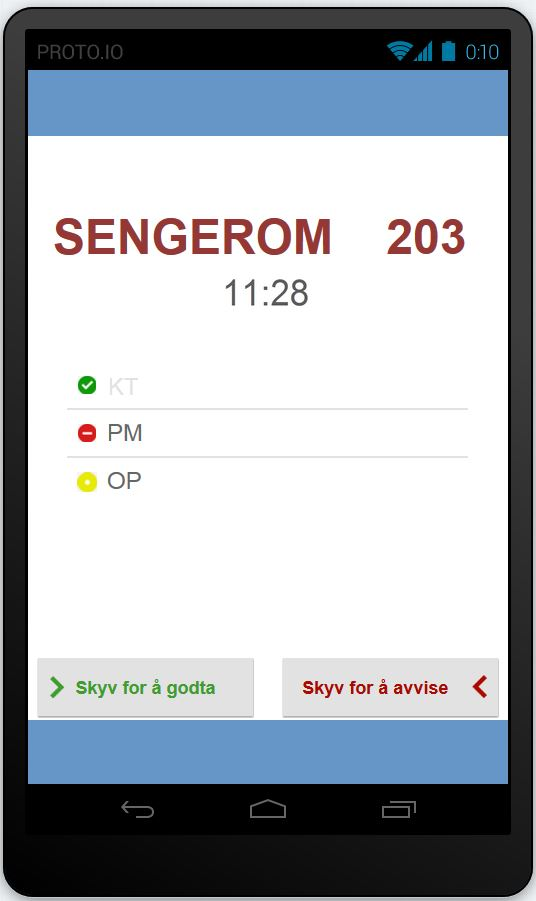
\includegraphics[scale=0.4]{proto_pasientsignal.jpg}
\caption{Skjermbilde ved inkommende pasientsignal. Her fra sengerom 203}
\label{protoPasientsignal}
\end{figure}

Med denne informsjonen umiddelbart tilgjengelig når en pasient ringer har sykepleieren mulighet til å, dersom han/hun ser at det er andre sykepleiere som er tilgjengelig, avvise anropet uten å være bekymret for at pasienten ikke får hjelp. Dette vil i andre omgang frigjøre kapasitet i arbeidsminnet (\ref{chp: kognisjon}) og dermed kan sykepleieren være mer mentalt tilstede hos pasienten som han/hun er hos på dette tidspunktet, som igjen gir bedre pasientomsorg.

\subsection{Skjermbildene og deres funksjon}

Som nevnt over er det paisentsignalet, og awareness-informsjonen som bilr kommunisert sammen med dette som er hovedfokuset i denne oppgaven. De øverige skjermbildene som her vil be presentert er laget av to grunner: de skal gi prototypen en mer helhetlig fremtoning, og de skal representere fremtidsrettet tankegang for fremtidig funksjonalitet, som kan være med å trigge kreativ tenkning hos deltagerene på workshoppene.

\subsubsection{Startsiden}
Forsiden er som ilustrert i figur \ref{proto_startside}. Knappen øverst til venstre gir tilgang til en dorp-down meny som vist i figur \ref{proto_startside_medMeny}. 

\begin{figure}[H]
	\centering
	\begin{subfigure}[b]{0.48\textwidth}
		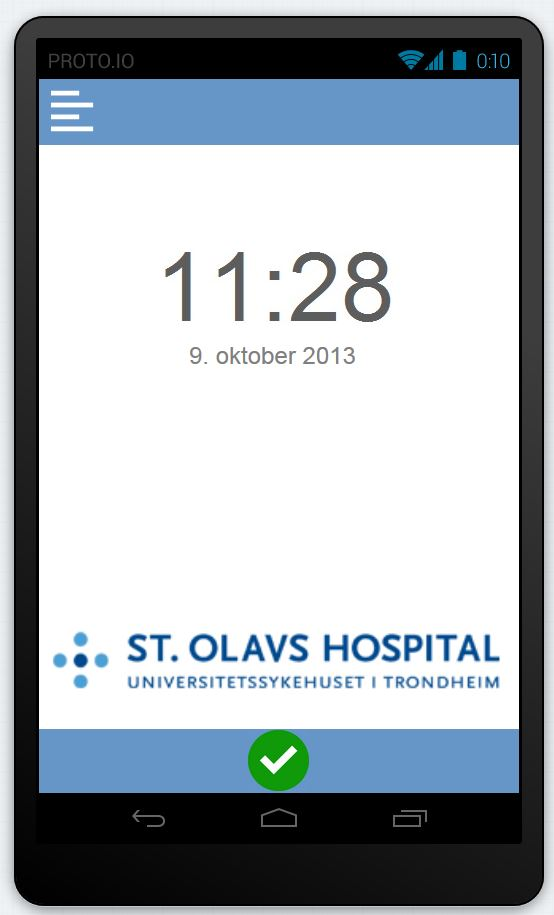
\includegraphics[scale=0.4]{proto_startside.jpg}
		\caption{Prototypens startside}
		\label{proto_startside}
	\end{subfigure}
	\begin{subfigure}[b]{0.48\textwidth}
		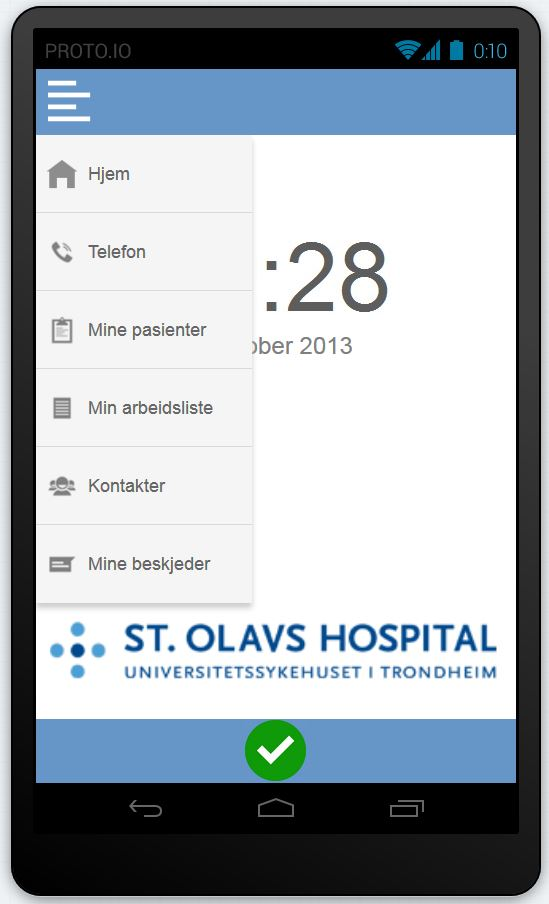
\includegraphics[scale=0.4]{proto_startside_medMeny.jpg}
		\caption{Prototypens startside med menyvisning}
		\label{proto_startside_medMeny}
	\end{subfigure}
	\caption{Prototypens startside}
\end{figure}

\noindent
Forsiden er ment som en standby-side, det vil si at det er denne siden som vises når skjermen slåes på. Tanken var at denne skal være enkel, med få elementer. Vi har derfor valgt kun klokke og datovisning i tillegg til status-indikatoren, midt på det nederste blå feltet (her illustrert med en grønn sirkel med hvit hake), og menyknappen øverst til venstre. Status-indikatoren og menyknappen vises på alle skjermbilder. 

\subsubsection{Min Arbeidsliste}
Her vises alle psientsignal du har godtatt, men ikke vært hos. Dette betyr at dersom du velger å godta et pasientsignal vil det legges i denne listen. Når du har gått inn på rommet hvor signalet ble utløst, vil elementet forsvinne fra listen. Dersom en sykepleier har godtatt flere psientsignal vil det da ligge flere elementer i listen. Dette er ment til å være til hjelp slik at sykepleieren ikke skal glemme noen av pasientene, selv om han/hun skulle bli avbrutt. Funksjonen vil på denne måten avlaste arbeidsminnet (se kapittel \ref{chp: kognisjon}) til sykepleierene slik at de kan være mer mentalt tilstede, og bedre kunne fokusere på oppgaven de holder på med.

\subsubsection{Mine Pasienter}
Dette er nok den funksjonen som er mest fremtidsrettet og åpen for mer informsjonsflyt slik prototypen står i dag. Sykepleierene fordeler pasientene mellom seg ved starten av hver vakt. Ved å registrere dette i bemanningsplanen (se appendiks \ref{appendix_dagenssystem}) vil disse legges i listen "Mine Pasienter". Her er ideen at det i fremtiden kunne være mulig å aksessere journaler, tidligere prøvesvar, samt få beskjed når nye prøvesvar er klare. Som vist i figur \ref{minePasienter}, kan nye blodprøvesvar da vasles og vises direkte på telefonen. Sykepleieren ser med én gang at det er kommet ny informasjon angående Hermansen. Ved å trykke på navnet hans ser man at varselet gjelder svar på blodprøvene, og ved å trykke på teksen "nye blodprøvesvar"\ vil svarene straks vises.

\begin{figure}[H]
\centering
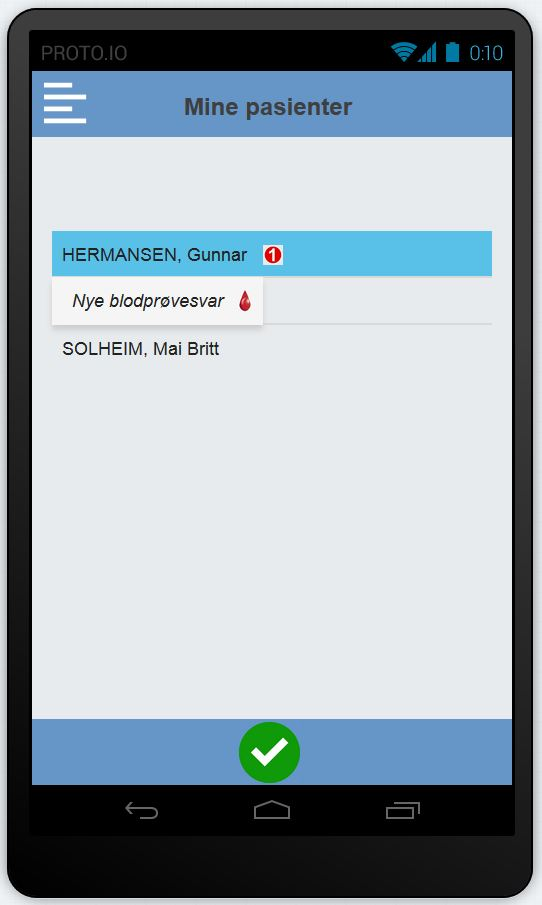
\includegraphics[scale=0.4]{minePasienter.jpg}
\caption{Eksempel på pasientlisten til en sykepleier. Her er det kommet svar på blodprøvende til Hermansen.}
\label{minePasienter}
\end{figure}

\subsubsection{Mine Beskjeder}
Mine beskjeder er en slags sms-lignende tjeneste hvor sykepleierene kan stille hverandre med spørsmål og gi beskjeder som ikke haster. Dette er en mindre forstyrrende og avbrytende måte å kommunisere på, når det ikke er avgjørende med rask respons.

\subsubsection{Kontakter}
Her vises kontaktinformasjon inkludert tilgjengelighet til de sykepleierene som er på jobb. Her skal det være enkelt å få oversikt over alle som er på vakt, og om de er tilgjengelige eller ikke. Dette er ment å brukes blandt annet dersom man har et spørsmål som flere kan svare på. Ved hjelp av kontaktlisten kan man velge den som mest sannsynlig vil bli minst forstyrret av henvendelsen. Ved å trykke på kontakten vil denne automatisk bli oppringt.

\subsubsection{Telefon}
Dette er den vanlige telefonfunksjonen vi kjenner fra vanlige telefoner, og trenger ingen detaljert forklaring.




\section{Workshopene}
\label{ws}

I denne delen vil vi legge frem funn vi gjorde i løpet av de to worshopene som ble holdt. Workshopene ble filmet, noe som har gitt oss muligheten til å gå tilbake å se på det utolkede materialet. Vi ønsket å finne ut av hvordan dagens system fungerer, hva som er positivt og hvilke utfordringer studentene opplever. Vi fant at det er behov for endringer av systemet, både med tanke på hvilken informasjon som formidles ved utløst signal, og hvordan dette formidles. Under gjennomgangen av prototypens funksjonalitet uttrykte flere av studentene at de syntes valgene vi hadde gjort var gode. Likevel fikk vi mange gode innspill, og studentene diskuterte potensielle utfordringer og kom med forslag til annen funksjonalitet. 


\subsection{Oversikt}
Det var ønskelig å avklare i hvilken grad sykepleierene har oversikt over inneliggende pasienter på sitt sengetun, og over kollegers ansvar og aktiviteter.

\noindent
Studentene fortalte at informasjon om pasientene og fordelig av ansvar blir nøye gjennomgått for de som går på vakt under vaktskiftemøtet, og at det er dette som er gunnlaget for oversikten gjennom vakten. Rapporteringen er nøyaktig nok til at du har oversikt over hvem alle pasientene er og endringer i deres tilstand fra dag til dag selv om du ikke har hovedansvar for gitte pasient. Det kom også frem at det etterstrebes at en pasient har samme primærsykepleier så godt det lar seg gjøre. Flere av deltagerene forteller at de har med seg en skriftlig oversikt over inneliggende pasienter, hvor detaljer fra vaktskiftemøtet noteres, og at denne kan brukes til oppslag gjennom dagen. Denne oversikten opprettholdes med mindre uforutsette hendelser oppstår, eksempelvis at pasienter bytter rom eller det kommer noen som må ha øyeblikkelig hjelp. 

\noindent
S1-A1 poengterer at selv om sykepleierene har oversikt over kollegers ansvar kan de ikke vite hvor alle er til en hver tid. Derimot vil kunnskapen om kollegenes ansvar gi en pekepinn på hvor det er sannsynelig å finne dem. I tillegg er det også utbredt bruk av telefon for å få tak i hverandre. 

\noindent
Når det kom til hvorvidt det var vanlig å si ifra til kolleger når man gå noe annet sted, for eksempel inn til en pasient, til et annet tun, avdeling eller etasje, eller til lunch viste det seg at dette var svært variabelt. Noen ville sagt ifra om de gikk inne til en pasient og ble borte en stund, samtidig som andre ikke ville gjort det da de regnet med at kolleger vet hva som skal gjøres på det gitte rommet og at det kan ta lengre tid.

\noindent
Dette var også tydelig under utspillingen av scenarioene uten prototype, hvor kun én av fire varslet sykepleieren tilstede på tunet om at hun skulle inn på et pasientrom. På spørsmål om man ville varslet andre før man går inn på et rom med en urolig pasient (noe som kan ta lengre tid) svarte S5-A3: \emph{"ja, man ville jo egentlig sagt det, men det er jo sjelden det blir sagt da, for de andre er jo gjerne klare over hva som skjer."}. Dette vitner om at sykepleierene regner med at alle har oversikt, både over hvilke pasienter som ligger på hvilke rom og hvem som har ansvar for de foskjellige pasientene.


\noindent
Etter introduksjon av prototypen, og muligheten til å sette sin status til  utilgjengelig for å formidle nettopp dette til kolleger så vi at dette var en funksjon som ble brukt i større grad enn å gi muntlig beskjed.
S1-A1 og S6-A4, som begge skulle utføre sårskift, benyttet seg av muligheten til å sette seg som utilgjengelig før de gikk inn til pasienten. S6-A4 valgte i tillegg å si ifra til sykepleieren på tunet om at hun ville være opptatt en stund. Da S2-A2, som skulle inn til en urolig pasient, ble spurt om hun ville sagt ifra til noen før hun gikk inn, svarte hun at: \emph{"hvis appen skal funke, burde man vel ikke trenge det."}, som vitner om rask adopsjon av funksjonen.

\noindent
For å forhindre at man blir stående som utilgjengelig når man ikke er det, noe som ville virke mot hensiktem med å gi sykepleierene bedre oversikt over kolleger, ble det foreslått forskjellige løsninger. (1) At systemet automatisk endrer status til tilgjengelig når man forlater rommet, (2) at telefonen gir en påminnelse om at man fremdeles står som utilgjengelig etter en viss tid, (3) at man har en tidsbegrensing på hvor lenge man kan stå som utilgjengelig.


\subsubsection{Håndtering av innkommende pasientsignal}
Under workshopene kom det også frem at sykepleierene tar hensyn til flere faktorer når de vurderer og håndterer innkommende pasientsignaler. 


\noindent
Alle deltagerene var klare på at dersom det var en pasient de selv hadde prismæransvar for ville de, dersom de hadde mulighet, gå til pasienten med en gang.
Flere av studentene fortalte også at de ved anrop fra en pasient de ikke er primær for, lar telefonen ringe en stund for å se om noen andre (hovedsaklig primærsykepleier) svarer. Dette til hensyn for pasienten, slik at denne skal slippe å forholde seg til flere sykepleiere enn nødvendig og for å klare å opprettholde oversikt over kolleger. I tilfeller hvor pasientsignalet ikke ble besvart ville noen av deltagerene gått til pasienten mens andre ville først hørt med eventuelle kolleger i nærheten om det ikke var noen av dem som har primæransvar for den aktuelle pasienten. Som ble poengtert av S1-A1 ville det ikke lenger være noen vits i fordelingen av pasienter mellom sykepleierene dersom alle svarer på alle anrop.

\noindent
En annen faktor som ble vektlagt var kunnskapen sykepleierene har om tilstanden til pasienten som har utløst signalet, og at dersom denne var dårlig ville de i større grad prioritere å se til pasienten fremfor å holde fast ved ansvarsfordelingen. 
Dersom sykepeieren befant seg sammen med en annen pasient når signalet ble utløst ville også tilstanden til denne tas i betraktning. 

\noindent
For å bedre kunne gjøre prioriteringer angående hvordan et pasientsignal skal behendles av den enkelte sykepleier var det stor oppslutting om forslaget å få et oversiktbilde av rommet hvor alarmen er utløst på telefonen slik at man kunne se pasienten, hvor i rommet denne befinner seg og hvordan det ser ut tul at vedkomne har det. Dette forslaget kom etter at vår prototype var introdusert som smarttelefon. Deltagerene kom også med forslag om å oppgi hvor i romemt signalet er utløst (ved sengen, ved døren, på toalettet osv.).

\subsection{Varsling fra telefon og veggpanel}

Det var også interessant å finne ut hvordan det innkommende pasientsignalet påvirker sykepleierenes arbeid. Det kom frem at de blir påvirket på svært forskjellige måter, noe som også kom tydelig frem under utspilling av scenarioene.
Der noen ble stresset ble andre ikke plaget overhodet. S4-A3 tenkte mest på hvordan det påvirket pasienten hun var hos, mens S9-A3 savnet å få en bekreftelse på at noen faktisk hadde gått inn til pasienten som utløste signalet slik at hun kunne slutte å tenke på det. 

\noindent
Det ble i flere anledninger de to dagene påpekt at det i visse situasjoner ville være positivt om telefonen ikke ringte like høyt, eventuelt kun vibrerte.
Dette var i stor grad av hensyn til pasientene. Flere av studentene opplevde at mange pasienter enten blir skremt av at det ringer, eller føler seg til bry og at de må forte seg å snakke ferdig. 
S2-A2 mente det er feil at pasientene må vise forståelse og godta at andre signaler skal forstyrre dem. Hun mente det er viktig at sykepleierene tar ansvar for at slike situasjoner blir håndtert på en god måte slik at pasientene ikke føler at de er til bry.
Dette ble begge dagene nevnt før prototypen med denne muligheten ble introdusert, men der var etter dette det var mest diskusjon rundt temaet. 
Det ble også foreslått at den ikke skulle gi fra seg noen form for vasling, men deltagerene kom da fort frem til at dette var lite hensikstmessig da de ønsket å ha en viss oversikt over hva som skjedde, eller «være med i loopen».

\noindent
I forbindelse med diskusjonen om hvordan man skal varsles når man har satt status til utilgjengelig kom det forslag om å flytte veggpanelet fra døren til veggen over sengen til pasienten. Dette gjalt speselt dersom det skulle vasles med svak eller ingen lyd, slik at man likevel ikke skal gå glipp av inkomne pasientsignaler.

\noindent
Også hvordan sykepleierenes status vil påvirke hvem som mottar pasientsignaler ble diskutert etter introduksjon av prototypen, og det kom flere forslag til hvordan dette kunne løses. Blant annet ble det foreslått at pasientsignaler først blir sendt til de som er tilgjengelige, deretter de som er opptatte, og eventuelt til slutt til de som er utilgjengelige. S2-A2 foreslo at de som er opptatt eller utilgjengelig først burde varsles med kun vibrasjon. Dersom signalet ble sendt til alle sykepleierene uten at det ble godtatt, burde derimot alle varsles med lyd.
\section{Resultatenes kvalitet}
\label{chp:analyse}

Vi valgte workshop som metode for datagenerering, da vi ønsket å avdekke brukerenes erfaringer og vurdering av det systemet de bruker i dag, samtidig som vi ønsket å teste vår foreslåtte løsning. Da vi i dette prosjektet har hatt en tidsbegrensning, var det ønskelig å generere data på en effektiv og produktiv måte \cite{Tjora}. Vi vil her vurdere forhold som kan ha påvirket datamaterialets kvalitet.

\subsection{Pålitelighet}
Hva angår materialets pålitelighet, vil vi her forsøke å redegjøre for de interne forholdene i forskningen som kan ha påvirket resultatene.

\subsubsection{Rollen som moderator}
Vi stilte selv som moderatorer under workshopenes fokusgruppediskusjoner, og dette var en ny erfaring for oss begge. At vi selv tok rollen som moderator ga oss god kontroll over hvilken retning samtalen tok, da vi kontrollerte hvilke spørsmål som ble stilt og når diskusjonen skulle avbrytes. Dette førte til at diskusjonen fokuserte på de temaene som var av relevans til våre forskningsspørsmål. På en annen side kan dette ha styrt diskusjonen i for stor grad, og det er en risiko for at interessant informasjon kunne kommet frem dersom diskusjonen ikke ble stoppet. Ved å stille detaljerte og gjentagende spørsmål kan man til en viss grad ha lagt ord i munnen på deltagerene. Da ingen av oss hadde hatt en slik rolle tidligere var det vanskelig å gjøre en god vurdering av hvorvidt vi klarte dette på en god måte underveis i workshopene. I ettertid kunne videoopptakene avdekke at det til tider ble stilt spørsmål som kan ha vært ledende, men inntrykket var likevel at informantene ikke lot seg påvirke av dette i vesentlig stor grad da de kom med flere innspill og nye ideer som vi som forskere ikke hadde vurdert selv.

\subsubsection{Rollen som fasilitator}
Den som hadde moderatorrollen hadde også rollen som fasilitator under utspillingen av scenarioene. Dette var i likhet med moderatorrollen en ny erfaring, og det var vanskelig å evaluere gjennomføringen underveis. Da vi hadde rollen som både fasilitator og forsker, var det utfordrende å opprettholde fullstendig nøytralitet, som påpekt av både Svanæs og Seland (2014) og Tjora (2012). Spørsmål kan derfor ha blitt stilt på en slik måte at det påvirket deltagerenes handlinger. Selv med videoopptak var det i ettertid vanskelig å avgjøre i hvor stor grad dette skjedde. 

\subsubsection{Deltagere på workshop}
I samråd med vår veileder kom vi frem til at vi trengte mellom tre og fem deltagere til hver workshop. Da vi hadde problemer med å få nok deltagere til å melde seg på, var vi i en situasjon hvor vi ikke kunne plukke ut deltagere for å få en representativ gruppesammensetning \cite{Seland, Cavaye95}. Som Berg (1999) beskriver, vil noen av utfordringene med CSCW-systemer være at systemer brukes av et bredt spekter av brukere. I 2006 hadde sykehuset 3263 ansatte sykepleiere \cite{nokkeltall}, og hvis vi antar at dette antallet ikke har blitt betraktelig mye lavere, kan man spørre seg hvorvidt ni deltagere kan representere et så stort antall sykepleiere, og om det i det hele tatt er mulig å inkludere alle i en slik prosess \cite{Cavaye95}. Ved å arrangere to uavhengige, men like, workshoper kunne vi sammenligne for å se om funnene varierte avhengig av individene som deltok. Som beskrevet av Berg (1999), man kan få kan feilaktige inntrykk basert på gruppesammensetning. I slike grupper er det en risiko for at noen individers meninger kommer tydeligere frem enn andres, og hvorvidt deltagerene faktisk var enige eller uenige var vanskelig å avgjøre. Alle deltagerene, med ett unntak, var kvinnelige studenter i samme aldersgruppe som oss. Det er derimot svært vanskelig å avgjøre om dette hadde påvirkning på resultatene. Det er også organisatoriske aspekter knyttet til deltagerenes medvirkning gjennom workshopene. Dersom vår løsning faktisk skulle blitt implementert, kunne deltagerenes mottakelse av systemet ved implementering, i stor grad avgjøres av deres individuelle forventninger til medvirkningen og dens utfall \cite{Jacobsen12, Cavaye95}. 

\subsection{Gyldighet}
Gyldighet knyttes til spørsmålet om resultatene vi kommer frem til faktisk svarer på forskningsspørsmålene vi har stilt. Dette kan styrkes ved at vi er åpne om hvordan forskningen er blitt gjennomført, og begrunnelser for de valgene som er tatt med tanke på metoder for datagenerering og teoretiske innspill til analysen. 

\subsubsection{Deltagerenes erfaringer}
Alle deltagerene var studenter, og hadde dermed begrenset erfaring med bruk av systemet vi ønsket å teste. Samtidig er de potensielle fremtidige brukere av pasientsignalsystemet, og vi anså derfor deres deltagelse som nyttig. Deltagerene hadde spesielt variert erfaring med bruk av telefon for mottak av pasientsignal. Dette førte til at en del av evalueringen ble synsing, og ikke direkte avledet fra eget bruk. Flere av studentene refererte i blant til hva de trodde de "vanlige" sykepleierene ville gjort, eller vanligvis gjør, i ulike situasjoner. Svanæs og Seland (2004) anbefaler at deltagerene har direkte erfaring med den type arbeid som skal utforskes. For å kunne evaluere utfordringer og fordeler med det eksisterende systemet og dagens arbeidspraksis, har det vært interessant å se hvordan bruk og rutiner varierer. 

\subsubsection{Kunstig situasjon}
Som påpekt av Alsos og Dahl (2008) er det viktig at de fysiske testomgivelsene, scenarioene og prototypene er så realistiske som mulig for å kunne generere gyldige resultater. Samtidig påpeker Berg (1999) at det for CSCW-systemer kan være vanskelig å gjenskape konteksten hvor systemet skal implementeres i et laboratorium. Det at workshopene ble holdt på NSEPs brukbarhetslab, et nytt og annerledes miljø for deltagerene, kan dermed ha påvirket workshopens realisme. På tross av at laboratoriet har flere rom, sykesenger, legefrakker og pasienttøy, samt våre mock-ups av forskjellige veggpaneler, kan det nye miljøet ha påvirket deltagerene. Den kunstige situasjonen kan ha gjort deltagerene mer bevisste på sine handlinger, og resultatene vil ikke nødvendigvis gjenspeile hva som er vanlig praksis. Det kan likevel hevdes å være en trygghet at alle deltagerene fikk observere de utspilte scenarioene, og kunne diskutere situasjonene i ettertid, og eventuelt kommentere hva man ville ha gjort annerledes. Det er naturligvis en risiko for at det man sier man ville gjort, ikke nødvendigvis gjøres i praksis, men totalt sett vil en slik felles diskusjon kunne avdekke reell arbeidspraksis i større grad. Deltagerene ble i etterkant av begge workshoper spurt hvorvidt de mente scenarioene var reelle og relevante, og alle deltagerene ga uttrykk for at de var det.

\subsubsection{Prototype og mock-ups}
Til tross for at vi poengterte at prototypen bare var skjermbilder med noe interaksjon, og ikke en operativ løsning, kan den ha fremstått som mer ferdig enn det den var, og dermed påvirket tilbakemeldigene fra deltagerene. Det kan ha hindret deltagerenes kreativitet, eller frahindret dem fra å komme med kritikk av hensyn til oss. Det at det eksisterende systemet ble forsøkt etterlignet med mock-ups på papir, og alle varslinger dermed ikke var slik de normalt er, kan ha påvirket workshopenes realisme.

\subsubsection{Problemer underveis}
Under WS2 oppsto det misforståelser under utspillingen av det første scenarioet, da deltageren som hadde rollen som sykepleier trodde det innkommende signalet på telefonen var et hasteanrop og ikke et vanlig pasientsignal. Dette førte til at valgene hun tok var annerledes enn det hun ellers ville gjort. Dette kunne gitt feilaktige resultater, hadde det ikke blitt avdekket. 

\subsection{Generalisering}
Det har i lenger tid pågått diskusjon om hvorvidt generalisering er nødvendig i kalitativ forskning, og i så fall hvordan dette skal gjøres. Generaisering beskriver i hvor stor grad resultatene er gyldige i andre situasjoner enn den som er studert. 

\chapter{Diskusjon}
\label{chp:diskusjon}
I denne delen vil vi diskutere funnene fra workshopene som ble holdt, i lys av teorien som er presentert i kapittel \ref{chp:teori}, og legge grunnlaget for å besvare forskningsspørsmålene indrodusert i kapittel \ref{chp:introduksjon}.

\section{Valg av teori}
Som nevnt i kapittel \ref{subsec:tidligereArbied} fikk vi innledningsvis utlvert flere artikler av vår veileder. Det er ikke til å komme forbi at disse satte utgangspunktet for veien videre. I hvor stor grad oppgaven ville tatt en annen retning dersom vi hadde tatt utgangspunkt i andre artikler er uvisst, men da vi allerede hadde en oppgavebeskrivelse å gå ut ifra ser vi det som usannsynlig at forskjellene ville vært store.
Der vi fant temaer vi ønsket å tilegne oss mer kunnskap om ble videre teori først valgt på bakgrunn av kildene til artiklene vi allerede hadde lest. Dersom det var behov for videre utfyllende teori tok vi i bruk Googles søkemotor Google Scholar, en søkemotor for akademisk litteratur. 

\noindent
Det har vært viktig for oss at kildene vi har valgt er pålitelige, og vi har dermed fosrsøkt å holde oss til artikler som er blitt publisert i tidsskrifter. Der det er brukt elektroniske kilder (nettsider) er dette dokumenter for spesifikke fakta om blandt annet St. Olavs Hospital, samt brukerveiledninger for pasientsignalsystemt som brukes i dag. 

\section{Prototypen}
\label{protoDisk}
Funksjonaliteten til prototypen ble i hovedsak basert på teori fra artiklene vi har lest, og hva vi utifra dette anså som mulige forbedringer. Vi fikk noe veiledning fra professor og veileder, men hadde ingen direkte innspill fra brukerene av systemet som grunnlag for valgene vi tok underveis.
Vi ønsket likevel å lage en prototyp til et system som ville blitt brukbart ved implementering (jf \ref{chp: brukbarhet}). Siden det var svært vanskelig å si hva brukeren forventet og hva som måtte til for å være effektiv i bruk, ble det mye synsing og bruk av det vi mente var sunn fornuft. Vi fokuserte på at all informasjon skulle være få trykk unna og at skjermbildene skulle ha samme oppbygning. Videre sørget vi for at viktig informasjon, som brukerens egen status, var direkte aksesserbart fra alle skjermbildene. 

\noindent
I dag brukes de trådløse enhetene i relativt liten grad for å støtte opp om awareness, da det er stort sett oversiktsbildet over på hvilke rom det er sykepleiere tilstede som brukes til dette. Med prototypen vi har laget er det lagt opp til langt mer omfattende bruk av de personlige enhetene til dette formålet. Det påpekes av Erickson og Kellog (2000) at sosialt translucent er en svært viktig egenskap ved et slikt system (jf \ref{awareness_CSCW}), noe vi vil argumentere for at vår prototype oppfyller.  Dersom en sykepleier setter sin status til utilgjengelig vil dette straks distribueres til kollegenes telefoner. På denne måten syneliggjøres det at de er engasjert i en aktivitet de ikke helst ikke vil forstyrres i. Dette gjør det mulig for andre sykepleiere å ta ansvarlige valg angående egne aktiviteter, samt i forhold til om se skal avbryte sykepleieren som er utilgjengelig. 

\noindent
Da det ikke var vår intensjon å teste skjermbildedesign til en slik enhet, la vi heller ikke vekt på bruk av teorier for dette. Likevel brukte vi tid på å lage et design vi trodde ville falle i smak hos deltagerene av workshopene. Dette var først og fremst for at dårlig design ikke skulle bli en faktor som påvirket tesingen av prototypens funktionalitet i stor grad. Om dette hadde noe for seg er det vanskelig å si noe om, men da dette ikke ble kommentert velger vi å anta at designet ikke var i veien for tesingen.

\section{Funn}

\subsection{Oversikt}
\label{oversikt}
Workshopene avdekket at sykepleierestudentene opplever at de har god oversikt over både pasienter og kolleger på tunet de jobber på. Ved vaktskiftet fordeles ansvar for pasientene, og informasjon om deres sykdomsbilde og tilstand blir gitt. Vi kan dermed argumentere for at vaktskiftemøtet resulterer i en form for kognitiv distribusjon, jf \ref{DistrKogn}, da sykepleierene som gruppe har større kapasitet til å holde en detaljert oversikt over pasientene, enn en sykepleier kan alene. Med kunnskapen sykepleierene tilegner seg ved dette møtet, oppstår redundans av funksjon, da flere sykepleiere kan hjelpe de samme pasientene. Vaktskiftemøtet resulterer også i sosial awareness, da sykepleierene får en indikasjon på hvilke aktiviteter deres kolleger vil delta i, og dermed hvor de sannsynligvis vil være å finne. Likevel poengterer S1-A1 at sykepleierene ikke vet hvor alle er til enhver tid, da det er stor variasjon i hvor vanlig det er å varsle andre om sine aktiviteter. Dette kan tyde på at sykepleierene ikke anser det som nødvendig å si i fra, da de antar at deres kolleger vet hva de gjør og hvor de er, selv om dette nødvendigvis ikke er tilfellet. Awareness slik det defineres innen CSCW, er å synliggjøre sine aktiviteter for, og oppfatte aktivitetene til kolleger, for å støtte opp om samarbeidet dem imellom. Ifølge Heath et al. (2002) og Schmidt (2002) oppnås denne typen awareness gjennom kontinuerlig interaksjon med andre. Vi ser derfor at vaktskiftemøtet fører til en viss sosial awareness, men at denne ikke alltid opprettholdes da det er variasjon i hvor stor grad man eksplisitt synliggjør sine aktiviteter. Ved gjennomgangen av pasientenes sykdomsbilde og tilstand, får sykepleierene et inntrykk av  hva som skal gjøres, eller hva som skjer på de forskjellige pasientrommene. Dette kan dermed tyde på at sykepleierene har god romlig awareness, såfremt det ikke oppstår situasjoner hvor pasienter bytter rom, eller uforutsette hendelser oppstår. Et eksempel på dette gis av S5-A3 som forklarer hvorfor man ikke sier i fra om at man skal inn på et rom hvor man kan bli værende en stund, med at de andre allerede er klare over hva som skjer. På samme måte tilegnes tidsmessig awareness gjennom denne oversikten som blir gitt over tidligere og planlagte aktiviteter, samt status quo. Vi ser dermed at de tre typene awareness Bardram et al. (2006) mener er de viktigste i helseomsorgen, til en viss grad er tilstede.

\noindent
Kognitive gjenstander, som tavler, lister og skjermer, beskrives som hensiktsmessige for å støtte deling og innhenting av informasjon. Sykepleierenes skriftlige oversikt over pasienter kan derfor sies å være en slik gjenstand, disse er derimot private og gir kun informasjon til de enkelte sykepleierene. Som et resultat av dette, oppstår redundans av data, da informasjon om pasientene finnes både i deres journaler, og notert i sykepleierenes lister. 

\subsection{Avbrudd og kognitiv kapasitet}
Da avbrudd kan være både positive og negative blir det viktig å gjøre en avveining i forhold til hvorvidt sykepleierene bør varsles, og eventuelt på hvilken måte dette bør gjøres. Under workshopene så vi at det var stor variasjon i hvordan sykepleierene ble påvirket av innkommende pasientsignaler. For hvert signal, måtte sykepleierene gjøre en vurdering på om de skulle bli, eller forlate pasienten de var inne hos. I tråd med Ebright (2010), som hevder at denne re-prioriteringen kan resultere i en kognitiv belastning som kan hemme oppmerksomheten, er det grunn til å anta at alle sykepleierene i større eller mindre grad blir påvirket av signalene. Det var derimot stor variasjon i hvorvidt sykepleierene selv opplevde å bli påvirket, da noen uttrykte at ikke lot seg påvirke, mens andre sa de ble stresset.

\noindent
Hvordan vasler og lyder kunne endres, og spesielt dersom sykepleieren valgte å sette sin status til utilgjengelig, ble derfor naturlig å diskutere under worskshopene. Grandhi og Jones (2010) beskriver fire teknikker for å håndtere avbrudd med hansikt å redusere negative effekter samtidig fom de positive effektene beholdes. Forslaget om å hoppe over sykepleiere med status utilgjengelig i første omgang kan knyttes opp mot teknikken forebygging, i form av at avbrytelsen da blir blokkert. Siden det ikke gis eksplisitt informasjon gjennom systemet om hva slags oppgave sykepleieren utfører, heller ikke informasjon om hva avbruddet gjelder, vil det ikke være aktuelt å kun tillate visse anrom basert på relevans i forhold til oppgave. Videre kan man si at muligheten til å sette status til utilgjengelig også vil ta i bruk teknikken fraråding, da symbolet som viser at en sykepleier er utilgjengelig og ønsker å ikke bli forstyrret implisitt fraråder andre sykepleiere å avbryte vedkomne. Her må hver enkelt selvfølgelig ta en vurdering på om innholdet i avbrytelsen er så viktig at det overgår den negative effekten ved avruddet. Endring i ringevolum fanges opp av teknikken modifisering, og reduserer interferensen mellom perseptuelle og kognitive prosesser til et minimum.
At sykeplierene vet hvilket rom som har utløst signalet, sammen med deres kunnskap om tilstanden til pasienten er viktig for hvordan de prioriterer signalet. Denne informasjonen fungerer da som en forhondsvisning. Selv om det i dette tilfellet ikke gir direkte informasjon angående hva signalet gjelder, vil romnummeret sammen med sykepleierens kunnskap om blandt annet pasientens tilastnad gi en indirekte indikasjon. Muligheten for å gå pasientene flere signalknapper for bruk ved forskjellige behov (som for eksempel drikke, toalettbesøk eller mer akutt hjelp), ble diskutert under workshopene, men deltagerene kom frem til at i tillegg til mulighet for misbruk fra pasientenes side, og faren for at sykepleierene skulle nedpriorietere signaler om mindre akutte behov, som drikke, er faren for at dersom en pasient skulle få et illebefinnende, og den første signalknappen denen fikk tak på var vannglasset kunne dette få fatale følger. Et annet forslag som kom frem på den andre dagen var et oversiktsbilde over rommet hvor signalet var utløst. Det var bred enighet om at dette ville være et godt grunnlag for å vurdere prioriteringen av signalet.   

\noindent
Etter introduksjon av prototypen, og muligheten til å sette sin status til utilgjengelig
for å formidle nettopp dette til kolleger så vi at dette var en funksjon som ble brukt
i større grad enn å gi muntlig beskjed. Det kan være flere grunner til dette, blandt annet at gjennom telefonen blir denne informasjonen distribuert til alle aktuelle sykepleiere, i stedet for bare dem som tilfeldigvis er tilstede der og da. Dette er også en mindre avbrytende måte å dele informasjon på, og er dermed med på å redusere mengden avbrytelser, som igjen kan hindre overbelastning av den enkeltes kognitive kapasitet. 

\noindent
Relasjonenen mellom sykepleieren som blir avbrutt av pasientsignalet og den pasienten som utløste signalet vil ha mye å si for hvordan sykepleieren prioriterer signalet. Dette er i tråd med Harr og Kaptelinins (2007) tanker om at oppførselen til avbryter og den avbrutte avhenger av mellommenskelige relasjoner. Selv om vi kan anta at pasientens adferd, eller valg om å avbrye eller ikke, ikke vil bli påvirket i nevneverdig grad i denne situasjonen, kom det tydelig frem under workshopene at dette for sykepleierene ofte er avgjørende for valget de tar i forhold til å besvare signalet eller ikke. 
Deres bekymring for hvordan den enkelte pasientent blir påvirket av at sykepleieren får et innkomne pasientsignal var tydelig. At også pasienten blir forstyrret når sykeplieren som er hos denne blir avbrutt, kalles av Harr og Kaptelinin (2007) for loksajonsbasert forstyrrelse. 


\chapter{Konklusjon}
\label{chp:konklusjon}
Vi fant at det er behov for endringer av systemet, både med tanke på hvilken informasjon som formidles ved utløst signal, og hvordan dette formidles.

flere "grunnsteiner" for awareness: Bardrams tre, to typer redundans(ifølge Cabitza kan awareness oppstå pga dette). -> godt grunnlag

%% include here the other chapters

\renewcommand*{\bibname}{Referanser}
\bibliographystyle{ieeetr}
\bibliography{ReferanseDatabase}

%% Uncomment the following if you have any appendix
\appendix
\addtocontents{toc}{%
\protect\vspace{1em}% 
\protect\noindent \bfseries \appendixtocname\protect\par
  \protect\vspace{-.5em}%
 }
 \renewcommand{\chaptername}{\appendixname}
%% include below possible appendices (chapters)
\chapter{Dagens pasientsignalsystem ved St. Olavs Hospital}
\label{appendix_dagenssystem}
Dette tillegget inneholder en beskrivelse av dagens pasientsignalsystem ved St.Olavs Hospital. Tekst og bilder er hentet fra opplæringsdokumenter og brukermanualer gitt ved St. Olavs Hospital, tilgjengelig på deres hjemmesider \cite{BrukerveiledningforPasientsignal, BrukermanualforPasientsignalogPasientsignalapplikasjon, BrukerveiledningforTradlostelefon}

\section{Dagens pasientsignalsystem}
Et signal utløses fra blant annet sengerom, fellesrom, stuer og toalett, for å tilkalle/alarmere pleiepersonell. Det skilles mellom to typer signaler: (1) Pasientsignal, som utløses av pasienten selv, og (2) hasteanrop, som utløses av pleiepersonell ved behov for umiddelbar assistanse. Pasientsignalsystemet er sammensatt av to integrerte systemer, et fast og et trådløst. 

\subsection{Pasientsignalanlegget - det faste systemet}
Det faste systemet, også refererert til som pasientsignalanlegget, består av fastmonterte paneler med trekksnorer og/eller trykknapper. Disse er illustrert i figur \ref{pasientsignalanlegget}.

\begin{figure}[H]
        \centering
        \begin{subfigure}[b]{0.3\textwidth}
        		\centering
                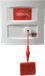
\includegraphics[scale=0.7]{anropspanel.png}
                \caption{Anropspanel}
                \label{anropspanel}
        \end{subfigure}%
        \begin{subfigure}[b]{0.3\textwidth}
        		\centering
                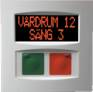
\includegraphics[scale=1.5]{rompanel.jpg}
                \caption{Rompanel}
                \label{rompanel}
        \end{subfigure}
        \begin{subfigure}[b]{0.3\textwidth}
        		\centering
                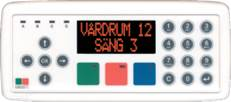
\includegraphics[scale=1]{vaktromsapparat.jpg}
                \caption{Vaktromsapparat}
                \label{vaktromsapparat}
        \end{subfigure}
        \caption{Pasientsignalanlegget}
        \label{pasientsignalanlegget}
\end{figure}

\noindent
\subsubsection{Anropspanelet}
Det finnes to typer anropspanel, et for våtrom og et for vanlig rom. I vanlige sengerom er anropspanelet plassert ved sengen, og har en trykknapp med lysdiode og en trekksnor.
Trykknappen utløser et hasteanrop, mens trekksnoren utløser et pasientsignal.

\subsubsection{Rompanelet}
Rompanelet er plassert ved døren til hvert av sengerommene på tunet. Det har et display, og en grønn og en rød trykknapp med hver sin lysdiode. Grønn knapp trykkes for å markere pleiepersonells tilstedeværelse eller for å avstille et signal. Rød knapp trykkes for å utløse pasientsignal, eller et hasteanrop dersom tilstedemarkering er aktivert. Rød knapp kan også holdes inne i 2 sekunder for å utløse hasteanrop, dersom tilstedemarkering ikke er aktivert. 

\subsubsection{Vaktromsapparatet}
Vaktromsapparatet er sentralt plassert i det åpne landskapet på sengetunet. Det består av et display og flere tall- og tegntaster. Displayet indikerer stedangivelse for et pasientsignal, hasteanrop og tilstedemarkerte rom. Pasientsignaler og hasteanrop er signalisert med rød tekst, mens tilstedemarkering er vist ved grønn tekst. Tall- og tegntastene brukes for å programmere apparatet.

\subsection{Det trådløse systemet}
Pasientsignalanlegget er videre tilkoblet det trådløse systemet, som består av følgende IKT-komponenter: pasientsignalapplikasjon, trådløs telefonenhet og pasientterminal, illustrert i figur \ref{pasientapplikasjon}, \ref{telefonenhet} og \ref{pasientterminal} henholdsvis.

\begin{figure}[H]
        \centering
        \begin{subfigure}[b]{0.35\textwidth}
        		\centering
                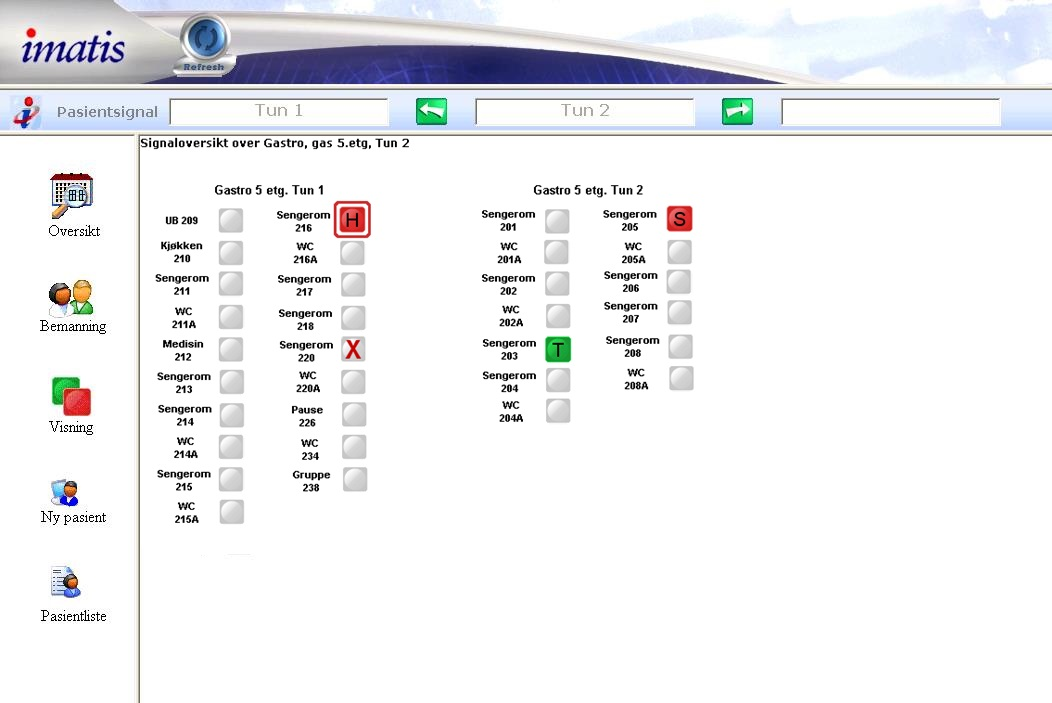
\includegraphics[scale=0.2]{pasientapplikasjon.jpg}
                \caption{Pasientsignalapplikasjon}
                \label{pasientapplikasjon}
        \end{subfigure}
        \begin{subfigure}[b]{0.35\textwidth}
        		\centering
                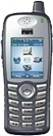
\includegraphics[scale=1]{telefon.jpg}
                \caption{Trådløs telefonenhet}
                \label{telefonenhet}
        \end{subfigure}
        \begin{subfigure}[b]{0.25\textwidth}
        		\centering
                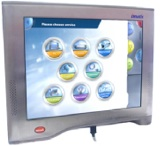
\includegraphics[scale=0.4]{pasientterminal.jpg}
                \caption{Pasientterminal}
                \label{pasientterminal}
        \end{subfigure}
        \caption{Det trådløse systemet}\label{dettradlosesystemet}
\end{figure}

\subsubsection{Pasientsignalapplikasjon}
Pasientsignalapplikasjonen kjører på en PC på hvert sengetun, 24 timer i døgnet, hver dag. Applikasjonen tilbyr i hovedsak fem funksjoner: (1) oversikt, (2) bemanning, (3) visning, (4) registrering av ny pasient og (5) en pasientliste. Vi vil her utdype funksjonene bemanning og visning, da disse er av mest relevans for vår oppgave.  

\noindent
Bemanningsplanen, vist i figur \ref{bemanningsplan}, knytter tilgjengelig pleiepersonell til rommene ved et sengetun. Pasientsignalene vil dermed sendes til riktig mottaker på bakgrunn av bemanningsplanen. For hvert rom vil det normalt tilknyttes en primærsykepleier og en disponibel sykepleier.

\begin{figure}[H]
\centering
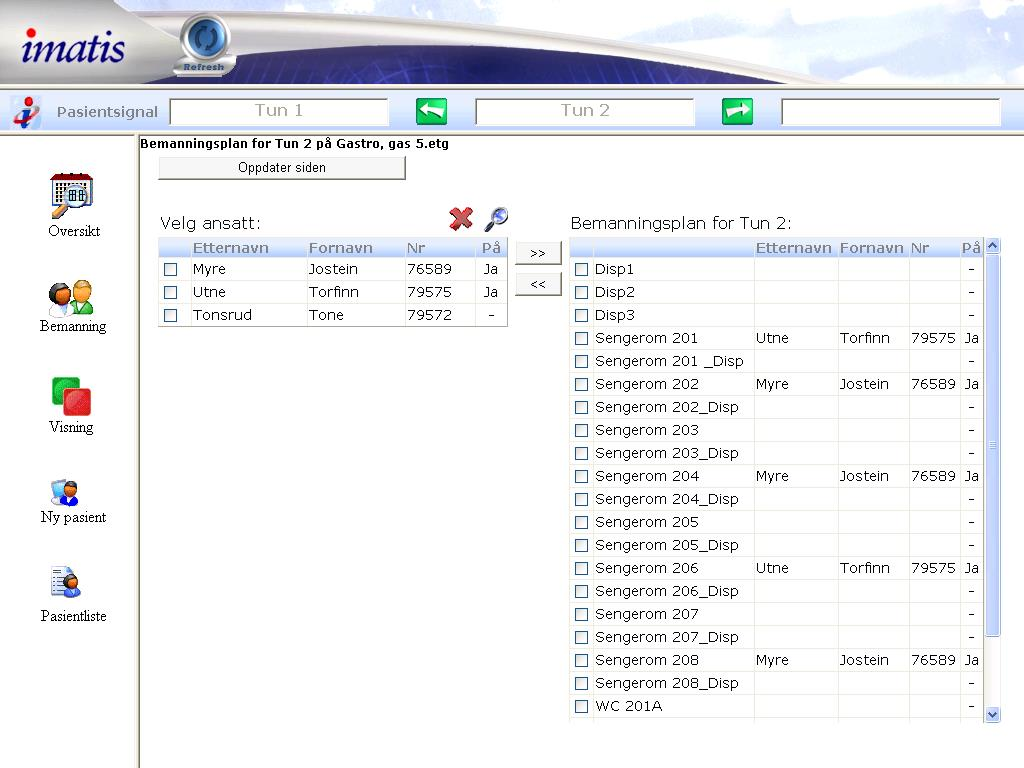
\includegraphics[scale=0.5]{bemanningsplan.jpg}
\caption{Bemanningsplan}
\label{bemanningsplan}
\end{figure}

\noindent
Funksjonen visning, vist i figur \ref{visning}, viser en oversikt over pasientsignalanlegget ved gjeldende sengetun, her vist som Gastro i 5. etasje, tun en og to. Grønn T markerer at pleiepersonell har trykket på den grønne knappen på rompanelet i det gjeldende sengerommet, og tilsynelatende er tilstede. Dette er ikke nødvendigvis riktig, da pleiepersonell kan glemme å trykke av den grønne knappen da de forlater rommet. Rød S signaliserer et pasientsignal, mens innrammet rød H signaliserer et hasteanrop. Rødt kryss varsler feil i systemet.

\begin{figure}[H]
\centering
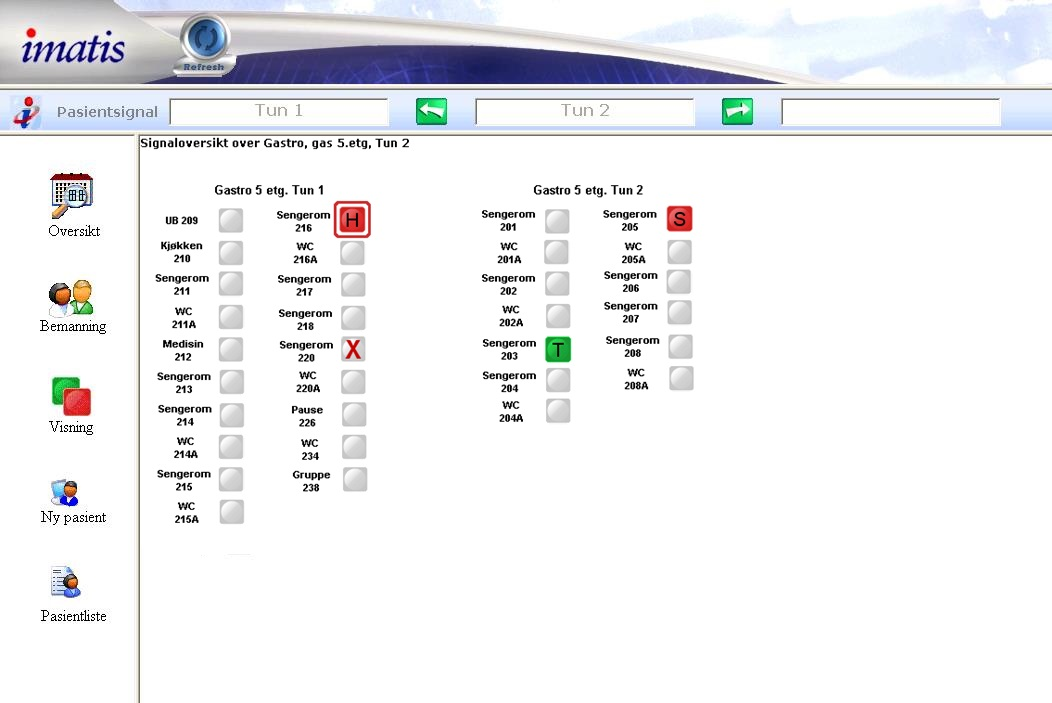
\includegraphics[scale=0.5]{pasientapplikasjon.jpg}
\caption{Visning}
\label{visning}
\end{figure}

\subsubsection{Trådløs telefonenhet}
De trådløse telefonenhetene inngår i det IP-baserte telefonisystemet ved St. Olavs Hospital, og er av typen Cisco Wireless IP Phone 7921G. I tillegg til å tilby basisfunksjoner som å ringe og sende tekstmeldinger, støtter de tjenester for alarmering. Pleiepersonell logger seg på telefonene for å motta pasientsignal og hasteanrop i forhold til ansvar gitt i bemanningsplanen.

\subsubsection{Pasientterminal}
Pasientterminalen inneholder en rekke funksjoner som pasienten kan benytte seg av, deriblant TV, radio, telefon, internett, spill og knapp for pasientsignal. Den røde knappen under skjermen benyttes for å utløse pasientsignal, og denne fungerer uavhengig av om terminalen er skrudd på eller ikke.

\pagebreak

\subsection{Hvordan det hele henger sammen}
\begin{figure}[H]
\centering
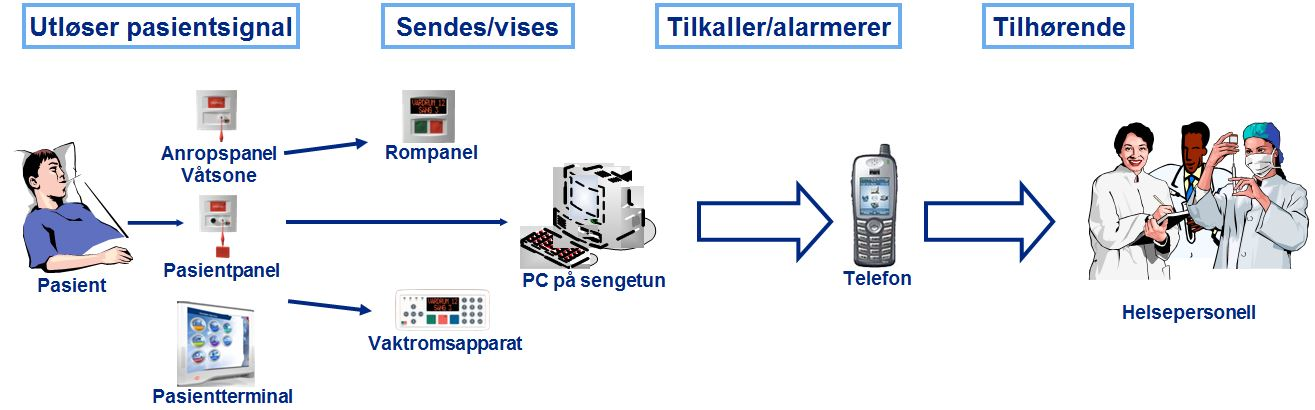
\includegraphics[scale=0.5]{alarmprosess.jpg}
\caption{Pasientsignal (Opplæring:Pasientsignal, delvis modifisert)}
\label{alarmprosess}
\end{figure}

\noindent
Pasienten kan utløse et pasientsignal ved å trykke på signalknappen på pasientterminalen, dra i snoren på anropspanelet, eller trykke på den røde knappen på rompanelet. Da vil lysdioden på rompanelet og anropspanelet blinke rødt. På andre sengerom hvor tilstedemarkering er aktivert vil lysdioden blinke rødt, og nummer- og stedsangivelse vil vises på displayet. Vaktromsapparatet vil blinke og avgi lydsignal, og pasientsignalapplikasjonen viser markering for pasientsignal.

\begin{figure}[H]
        \centering
        \begin{subfigure}[b]{0.35\textwidth}
        		\centering
                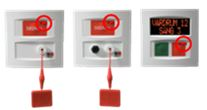
\includegraphics[scale=0.7]{signal_paneler.jpg}
        \end{subfigure}
        \begin{subfigure}[b]{0.35\textwidth}
        		\centering
                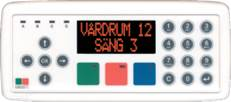
\includegraphics[scale=1]{vaktromsapparat.jpg}
                \label{telefon}
        \end{subfigure}
        \caption{Alarmering ved pasientsignal}\label{pasientsignalalarm}
\end{figure}

\begin{figure}[H]
\centering
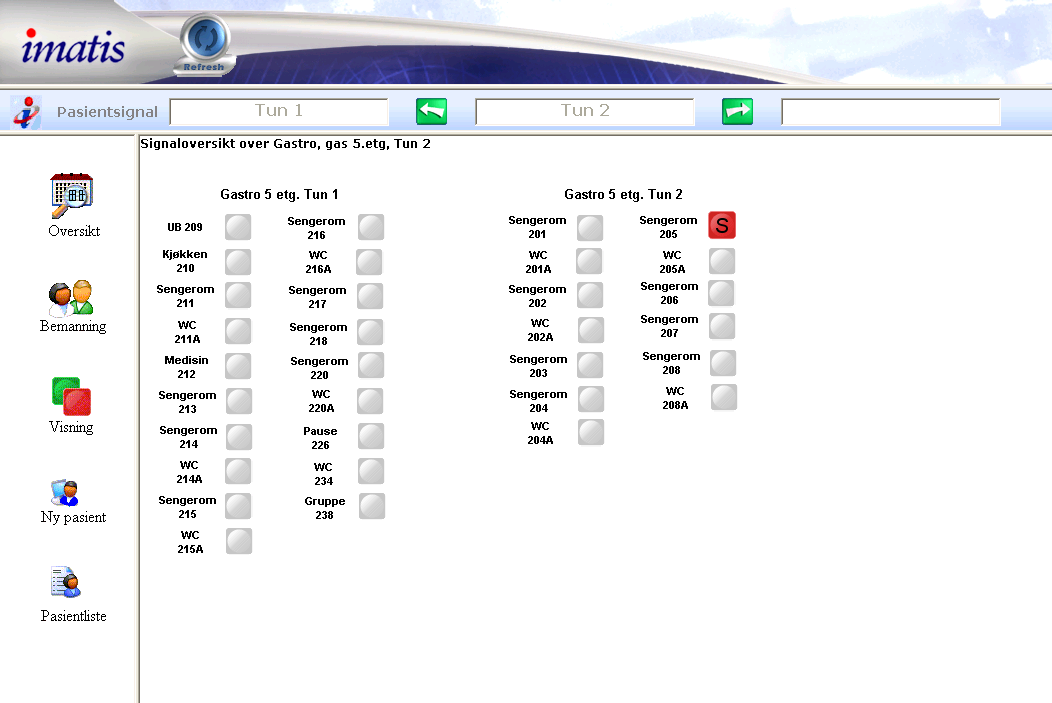
\includegraphics[scale=0.4]{applikasjonalarm.png}
\caption{Pasientsignalapplikasjon ved alarm (Brukermanual for Pasientsignal og Pasientsignalapplikasjon )}
\label{alarmprosess}
\end{figure}

\noindent
Dedikert pleiepersonell registrert i bemanningsplanen tilkalles på sin trådløse telefonenhet ved at melding vises på displayet, og lydsignal avgis. Mottaker har da mulighet til å godta eller avvise pasientsignalet. Dersom vedkommende velger å avvise tilkallingen, eller ikke foretar seg noe innen 15 sekunder, vil signalet sendes videre til neste ressurs. Slik vil det fortsette inntil tilkallingen blir bekreftet.

\begin{figure}[H]
\centering
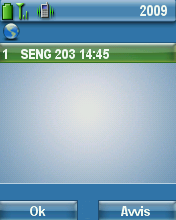
\includegraphics[scale=1]{alarmtelefon.png}
\caption{Trådløs telefonenhet ved alarm (Opplæring: Pasientsignal)}
\label{alarmprosess}
\end{figure}

\noindent
Dersom mottaker godtar tilkallingen vil den legges i mottakers arbeidsliste, og vedkommende har 2 minutter på seg for å tilstedemarkere seg på rommet, ellers vil tilkallingen videresendes til neste registrerte ressurs.

\begin{figure}[H]
\centering
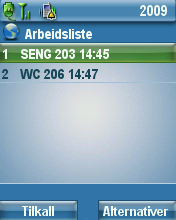
\includegraphics[scale=1]{telefonok.png}
\caption{Arbeidsliste (Opplæring: Pasientsignal)}
\label{alarmprosess}
\end{figure}

\noindent
Ved tilstedemarkering vil lyssignalet stoppe på anropspanelene, og rompanelet vil blinke med grønt lys. Vaktromsapparatet viser sengenummer og stopper lydsignalet, tilkallingen fjernes fra mottakers arbeidsliste, og pasientsignalapplikasjonen viser tilstedemarkering.
 
\begin{figure}[H]
        \centering
        \begin{subfigure}[b]{0.35\textwidth}
        		\centering
                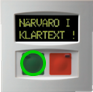
\includegraphics[scale=1]{rompanelok.png}
                \caption{Rompanel}
                \label{rompanelok}
        \end{subfigure}
        \begin{subfigure}[b]{0.25\textwidth}
        		\centering
                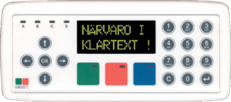
\includegraphics[scale=0.9]{vaok.png}
                \caption{Vaktromsapparat}
                \label{vaok}
        \end{subfigure}
        \caption{Det faste systemet etter tilstedemarkering}
\end{figure} 

\begin{figure}[H]
\centering
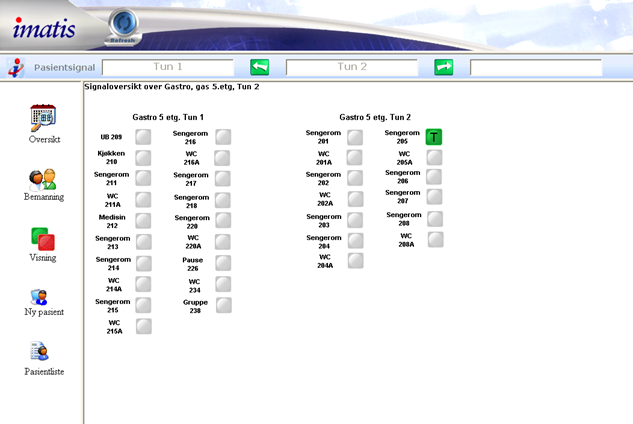
\includegraphics[scale=1]{applikasjonok.png}
\caption{Pasientsignalapplikasjon etter tilstedemarkering}
\label{applikasjonok}
\end{figure}

\noindent
Pleiepersonell trykker på den grønne knappen for å avstille pasientsignalet. Dersom pleiepersonell får behov for assistanse kan han/hun utløse et hasteanrop ved å bruke signalknappen på anropspanelet eller den røde knappen på rompanelet. Alarmen indikeres ved et hastig lydsignal, og røde tall for romnummer og stedsangivelse blinker hurtig på vaktromsapparatet og tilstedemarkerte rompaneler. På det gjeldende rommet vil både rød og grønn lysdiode blinke på rompanelet. I tillegg sendes en hasteanropsmelding, som ikke kan avvises, til samtlige av pleiepersonellets trådløse telefoner på sengetunet. Pasientsignalapplikasjonen viser markering for hasteanrop. Hasteanrop legges i arbeidsliste og avstilles på samme måte som pasientsignaler.

\begin{figure}[H]
\centering
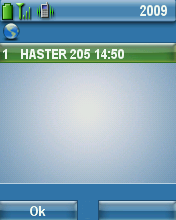
\includegraphics[scale=1]{hasteanropsmelding.png}
\caption{Trådløs telefonenhet ved hasteanrop}

\begin{figure}[H]
\centering
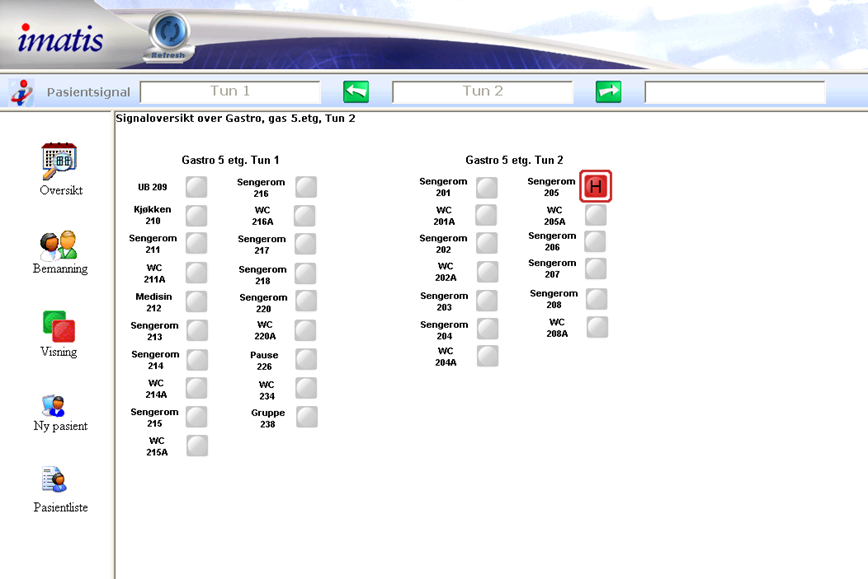
\includegraphics[scale=1]{applikasjonhast.png}
\caption{Pasientsignalapplikasjon ved hasteanrop}
\label{applikasjonok}
\end{figure}
\label{applikasjonok}
\end{figure}











\chapter{Plan for Workshop}
\label{appendix_workshop}


\textbf{Dette gjøres på forhånd:}
\begin{itemize}
  \item Klargjøre laben og artefakter
  \item Lage navneskilt
\end{itemize}

%\begin{adjustbox}{with=\textwith, hight=\texthight}
\begin{table}[H]
%\small
\caption{Overordnet plan for dagen}
%\centering
\begin{tabular}{l|l|l|l|l}
\hline
\textbf{\begin{tabular}[x]{@{}c@{}}Del av\\workshop\end{tabular}} & \textbf{Beskrivelse} & \textbf{Hvor} & \textbf{Tidspunkt} & \textbf{Varighet}\\
\hline
Steg 1 & Informasjon & \begin{tabular}[x]{@{}c@{}}Rundt bord\\/i gangen\end{tabular} & 13:00-13:15 & 15min\\
\hline
Steg 2 & Fokusgruppe med scenarier & \begin{tabular}[x]{@{}c@{}}Rundt bord\\/i gangen\end{tabular} & 13:15-13:45 & 30min\\
\hline
& \textbf{Pause} & & 13:45-13.50 & 5min\\
\hline
Steg 3 &\begin{tabular}[x]{@{}c@{}} Scenarioer med rollespill\\- uten prototype\end{tabular} & Inne på sengerom & 13:50-14:25 & 35min\\
\hline
& \begin{tabular}[x]{@{}c@{}}Scenarioer med rollespill\\- med prototype\end{tabular} & Inne på sengerom & 14:25-15:00 & 35min\\
\hline
& \textbf{Pause} & & 15:00-15:15 & 15min\\
\hline
Steg 4 & Fokusgruppe/oppsummering & \begin{tabular}[x]{@{}c@{}}Rundt bord\\/i gangen\end{tabular} & 15:15-16:00 & 45min
\end{tabular}
\label{OverordnetPlan}
\end{table}
%\end{adjustbox}

\pagebreak

\textbf{Forskningsspørsmål:}
\begin{enumerate}
  \item Identifisere behov knyttet til funksjonalitet for støtte av distribusjon av awareness-informasjon.
  \item Hvordan kan systemet endres for å begrense potensielle negative effekter ved avbrytelser?
\end{enumerate}

\subsubsection{Steg1: Informasjon - 13:00-13:15 (15min)}
\begin{itemize}
  \item Ønsker velkommen
  \item Presentasjonsrunde
  \item Presentasjon av roller (fasilitator, pasienter etc\ldots)
  \item Presenterer planen for workshopen og dens hensikt
  \begin{itemize}
  \item Vil vil først ha en felles diskusjon her, hvor vi ønsker å avdekke dagens situasjon mtp ansvarsfordeling og organisering av arbeidet
  	\item Vi vil deretter spille ut et par scenarioer på sengerommene her, hvor dere bruker de telefonene og funksjonene dere er vant med
  	\item Deretter vil vi forklare funksjonaliteten til prototypen vi har laget, for så å spille ut et par scenarier hvor vi ønsker at dere skal bruke denne
  	\item Til sist ønsker vi en oppsumering/diskusjon rundt disse scenarioene og deres syn på prototypen
  \end{itemize}
\end{itemize}

\noindent
Vi ønsker at alle bidrar i alle diskusjonene. Vi er her fordi vi ønsker å høre deres tanker/meninger

\subsubsection{Steg 2: Fokusgruppe med scenarioer}

\begin{table}[H]
\small
\caption{Scenarioer til fokusgruppe}
\begin{tabular}{p{4cm}|p{5cm}|l|l}
\hline
\textbf{Scenario} & \textbf{Oppfølgingsspørsmål} & \textbf{Tidspunkt} & \textbf{Varighet}\\
\hline
\emph{Rollen som primærsykepleier:} Du har ansvar for to av pasientene på tunet. \textbf{Hvordan vil du definere/beskrive denne rollen?} & I hvilken grad kjenner du til de andre pasientene? \begin{itemize}
\item Hvem har ansvar?
\item sykdomsbilde og tilstand
\item lokasjon
\item hvem og hvilket type rom
\end{itemize}
& 13:15-13:25 & 10min\\
\hline
\emph{Rollen som disp:} Du er disp for to av pasientene på tunet. \textbf{Hvordan vil du definere/beskrive denne rollen?} & I hvilken grad påvirker det beslutningen du tar om å svare på et pasientsignal, når du får et anrop fra en pasient du er disp for?
 & 13:25-13:35 & 10min\\
\hline
\emph{Utilgjengelig:} Du havner i en situasjon hvor du vil være utilgjengelig i en periode.
\begin{itemize}
\item i hvilke situasjoner er det ønskelig å kunne være “utilgjengelig” for henvendelser?
\item Hvilke henvendelser vil du ønske å motta uansett situasjon?
\item Hvilke henvendelser vil du helst ikke motta? Hvorfor?
\end{itemize}
& 
\begin{itemize}
\item Hvem informeres (kolleger/pasienter)?
\item Hva med telefonen?
\item Endres bemanningsplanen?
\item Lunchpause?
\item sårskift?
\item Urolig psient?
\item Andre situasjoner?
\end{itemize}
& 13:35-13.45 & 10min\\
\end{tabular}
\label{Steg2}
\end{table}

\textbf{Pause - 5min}
\pagebreak
\subsubsection{Steg 3: Scenarioer med rollespill}



\begin{itemize}
\item Presentasjon av pasientenes sykdomshistorier rundt bordet før vi starter rollespillene
\end{itemize}

\begin{table}[H]
\small
\caption{Scenario 1 for pasientsignal uten prototype}
\begin{tabular}{p{3cm}|p{2cm}|p{4cm}|l|l}
\hline
\textbf{Scenario} & \textbf{Aksjon} & \textbf{Oppfølgingsspørsmål} & \textbf{Tidspunkt} & \textbf{Varighet}\\
\hline
Du står i gangen, en annen sykepleier er også til stede. Du skal inn til Jonas fordi du vet han er veldig usikker og bekymret, og vil høre hvordan det går & & Hva slags forberedelser gjør du og hvorfor? (sier du fra til andre?)
& 13:50-13:55 & 5min\\
\hline
Du er inne hos Jonas og har en seriøs samtale om hans tilstand & Adam utløser pasientsignal. & 
\begin{itemize}
\item Hva gjør du?
\item Hvor ser du?
\item Ønsker du å fortsette samtalen uavbrutt eller forlater du rommet?
\item Hvordan påvirker signalet situasjonen?
\item Hvilken informasjon ville satt deg i bedre stand til å ta en avgjørelse?
\item Hvis du ikke velger å forlate rommet, hvorfor blir du?
\item Dersom du forlater rommet, og det viser seg at Adam ønsket et glass vann, føler du at du tok riktig avgjørelse?
\end{itemize}
 & 13:55-14:00 & 5min\\
\end{tabular}
\label{Steg3.1}
\end{table}

\begin{table}[H]
\small
\caption{Scenario 2 for pasientsignal uten prototype}
\begin{tabular}{p{3cm}|p{2cm}|p{4cm}|l|l}
\hline
\textbf{Scenario} & \textbf{Aksjon} & \textbf{Oppfølgingsspørsmål} & \textbf{Tidspunkt} & \textbf{Varighet}\\
\hline
Du står i gangen, en annen sykepleier er også til stede. Du skal inn til Adam for å utføre sårskift, og har kledd deg opp med stellefrakk  mm. & & Hva slags forberedelser gjør du og hvorfor? (sier du fra til andre?)
& 14:05-14:10 & 5min\\
\hline
Du er inne hos Adam og Utfører sårskift & Jonas utløser pasientsignal. & 
\begin{itemize}
\item Hva gjør du?
\item Hvor ser du?
\item Ønsker du å fortsette sårskiftet eller forlater du rommet? Hvilke faktorer spiller inn?
\item Hvordan påvirker signalet situasjonen?
\item Hvordan blir arbeidet påvirket?
\item Ville du satt deg som utilgjengelig? Sagt fra til noen om at du skal foreta et sårskift?
\item Dersom du forlater rommet, og det viser seg at Jonas ønsket et glass vann, føler du at du tok riktig avgjørelse?
\end{itemize}
 & 14:10-14:25 & 15min\\
\end{tabular}
\label{Steg3.2}
\end{table}

\pagebreak

\begin{table}[H]
\small
\caption{Scenario 1 for pasientsignal med prototype}
\begin{tabular}{p{3cm}|p{2cm}|p{4cm}|l|l}
\hline
\textbf{Scenario} & \textbf{Aksjon} & \textbf{Oppfølgingsspørsmål} & \textbf{Tidspunkt} & \textbf{Varighet}\\
\hline
Du er inne hos Jonas og har en seriøs samtale om hans tilstand & Adam utløser pasientsignal & \begin{itemize}
\item Hva gjør du?
\item Hvor ser du?
\item Ønsker du å fortsette samtalen uavbrutt eller forlater du rommet? Hvilke faktorer spiller inn?
\item Hvordan påvirker signalet situasjonen?
\item Hvordan blir arbeidet påvirket?
\item Hvis du ikke velger å forlate rommet, hvorfor blir du?
\item Dersom du forlater rommet, og det viser seg at Adam ønsket et glass vann, føler du at du tok riktig avgjørelse?
\item Ville du brukt “kontakter” for å se de andre sin status
\item Om du merker at Jonas trenger at du er der en stund, ville du satt deg som opptatt? (rød)
\item Kommentarer til design?
\end{itemize}
& 14:25-14:40 & 15min\\
\end{tabular}
\label{Steg3.3}
\end{table}

\begin{table}[H]
\small
\caption{Scenario 2 for pasientsignal med prototype}
\begin{tabular}{p{3cm}|p{2cm}|p{4cm}|l|l}
\hline
\textbf{Scenario} & \textbf{Aksjon} & \textbf{Oppfølgingsspørsmål} & \textbf{Tidspunkt} & \textbf{Varighet}\\
\hline
Du er inne hos Adam og utfører sårskift. & Jonas utløser pasientsignal. \emph{Telefonen vibrerer} & \begin{itemize}
\item Hva gjør du?
\item Hvor ser du?
\item Ønsker du å fortsette sårskiftet eller forlater du rommet? Hvilke faktorer spiller inn?
\item Hvordan påvirker signalet situasjonen?
\item Hvordan blir arbeidet påvirket?
\item Hvis du ikke velger å forlate rommet, hvorfor blir du?
\item Ville du satt deg som utilgjengelig? Sagt fra til noen om at du skal foreta et sårskift?
\item Ville du brukt “kontakter” for å se de andre sin status
\item Kommentarer til design?
\end{itemize}
& 14:40-15:00 & 20min\\
\end{tabular}
\label{Steg3.4}
\end{table}

\textbf{Pause - 15min}

\pagebreak

\subsubsection{Steg 4: Fokusgruppe/Sammendrag - 15:15-16:00 (45min)}

\begin{itemize}
\item Oppsummering av scenarioene
	\begin{itemize}
	\item Var situasjonene som ble utspilt relevante? Eventuelt hvorfor ikke?
\item Forslag til oppfølgingsspørsmål:
	\item Tror dere noe av den løsningen vi foreslo kan være av nytte?
	\item Kan dere se for dere noe sånt i bruk?
	\item I forhold til å ta avgjørelsen om dere skal forlate pasienten til fordel for pasienten som ringer - synes dere prototypen ga tilstrekkelig informasjon?
		\item Er det annen informasjon dere kunne tenke dere?
	\item Tror dere informasjonen prototypen gir vil gjøre avbrytelsene mindre forstyrrende?
	\item Tror dere funksjonen om tilstedeværelsen til andre sykepleiere vil gjøre avbrytelsene mindre forstyrrende?
	\end{itemize}
\end{itemize}
\include{appendix_pasientbeskrivelser}
\include{appendix_sporreskjema}


\end{document} 
